%%%%%%%%%%%%%%%%%%%%%%%%%%%%%%%%%%%%%%%%%%%%%%%%%%%%%%%%%%%%%%%%%%%%%%%%
% Golden Sacra - Memoria
% Escuela Politécnica Superior de la Universidad de Alicante
% Realizado por: Ángel Jesús Terol Martínez
% Contacto: jtm37@alu.ua.es
%%%%%%%%%%%%%%%%%%%%%%%%%%%%%%%%%%%%%%%%%%%%%%%%%%%%%%%%%%%%%%%%%%%%%%%%
\chapter{Desarrollo}
\label{ep:development}

\section{Iteración 0 - Iniciación en la Programación para Game Boy}

Esta iteración dio \textbf{comienzo} de manera \textbf{previa a la propuesta de TFG}, con la idea de ir preparado al inicio de desarrollo y llevar los conceptos básicos aprendidos. Esto \textbf{ha ayudado a conocer} mejor \textbf{cómo ensamblar} un trozo de código (y hacerlo funcionar en una GB real) o \textbf{cómo meter un sprite en memoria y moverlo por pantalla}.

\subsection{Hello World}

El \textbf{primer experimento} que se ha conseguido desarrollar ha sido el de mostrar por pantalla el conocido \textbf{"Hello World"} que todos hemos programado alguna vez al empezar con un lenguaje nuevo. A pesar de tener "basura visual", se podían llegar a distinguir las letras.

\begin{figure}[h]
\centering
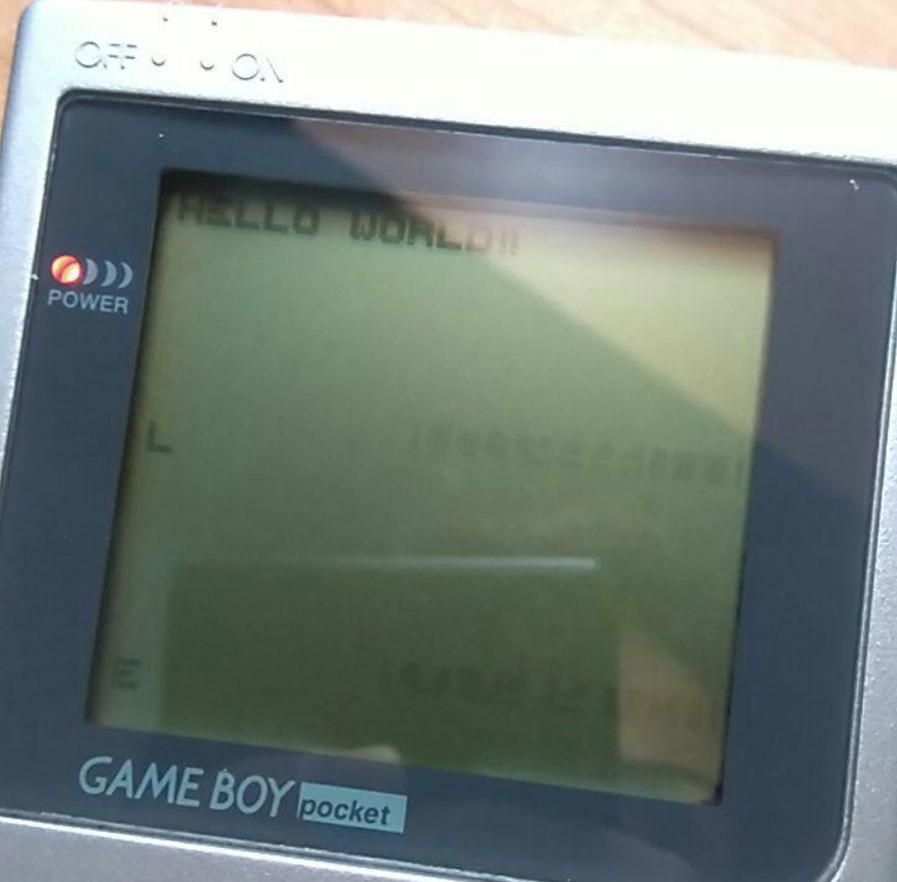
\includegraphics[width=0.5\textwidth]{include/images/desarrollo/hello_world.png}
\caption{Hello World}
\label{figure:hello_world}
\end{figure}

No tiene mucho misterio: primero de todo \textbf{cargamos en memoria los tiles correspondientes}, que en este caso no eran otros que las letras del abecedario inglés. Lo segundo que necesitamos es \textbf{introducir en memoria de vídeo (OAM) los sprites que consideremos oportunos manualmente}, uno tras otro, y dejando entre ellos una separación de 8 pixels (recordemos que cada tile son 8x8 pixels).
\\ \\
¿Cómo y dónde se deben cargar los tiles para posteriormente utilizarlos? Si observamos el mapa de memoria (\hyperref[memory_map]{9.2}), comprobaremos que la posicion \textbf{\$8000} hace referencia a la VRAM interna. Y precisamente es aquí donde \textbf{la consola busca el tile correspondiente cada vez que insertemos un sprite en la OAM}.
\\
El método que a crear es el equivalente al \textit{ldir} de \textit{Amstrad}, con el que podremos \textbf{insertar filas de bytes de un origen a un destino de forma directa}.

\begin{lstlisting}[caption={Copia de Memoria}, label={code:copy_mem}]
COPY_MEM:
	ld 	 a, [hl]			; cargamos el dato en A
	ld	 [de], a			; copiamos el dato al destino
	dec	 bc					; uno menos por copiar
							
	ld	 a, c				; comprobamos si bc es cero
	or	 b
	ret	 z					; si es cero, volvemos
	
	inc	 hl
	inc	 de
	jr	 RS_COPY_MEM

\end{lstlisting}

La función tiene como \textbf{parámetros} la \textbf{dirección origen} en el registro HL, la \textbf{dirección destino} en DE, y el \textbf{número de bytes} a copiar en BC. Simplemente va insertando en HL el contenido de DE, incrementa ambas direcciones, decrementa el contador para saber si aún quedan bytes restantes por copiar y, si no es así, terminar y volver.
\\ \\
Lo siguiente es \textbf{saber cómo crear un sprite} por cada letra que se desee mostrar:
\\ \\
Como ya se ha visto en el \textbf{apartado} \hyperref[manual_sprites]{\textbf{7.4}}, lo que debemos hacer es \textbf{indicar el sitio en el que lo queremos} y \textbf{qué número de tile mostrar} (del atributo no nos vamos a preocupar de momento, por lo que lo dejamos a nulo). Estos datos se van a guardar en cualquier lugar de la ROM (según vea conveniente el ensamblador) para, una vez ejecutado el juego, leer y copiarlos.

\begin{lstlisting}[caption={Inserción de un Sprite a la OAM}, label={code:spr_oam}]
MAKE_LETTER:
	ld 	 hl, letter_H
	ld 	 de, _VRAM
	ld 	 bc, $4
	jp 	 RS_COPY_MEM

letter_H: 	DB 5, 5, 7, 0

\end{lstlisting}

Con este ejemplo ya aparecerá la letra H por pantalla. Destacar que el código es muy mejorable ya que \textbf{no es reescalable} y habría que tener el mismo trozo de código para cada letra que queramos meter en RAM.
\\ \\
También dejar claro que el mensaje de "Hello World" \textbf{podría haberse hecho sin utilizar RAM} (simplemente insertándolo de background) ya que no se va a modificar en ningún momento. Se ha realizado de esta forma, de todos modos, para facilitar explicaciones futuras.

\subsection{Sprites y Scroll}

La \textbf{segunda prueba} se basó en conseguir \textbf{animar y mover un sprite por pantalla} y \textbf{aprender el funcionamiento del scroll}.

\begin{figure}[h]
\centering
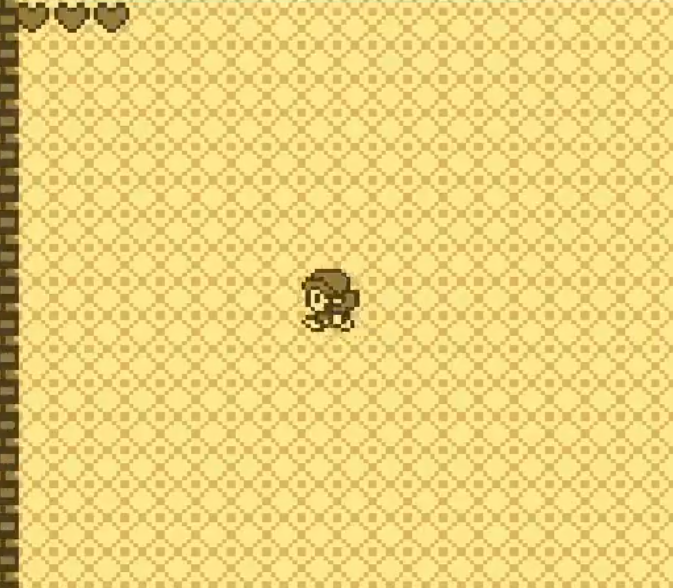
\includegraphics[width=0.5\textwidth]{include/images/desarrollo/sprite_scroll.png}
\caption{Sprite Animado en NO\$GMB}
\label{figure:sprite_scroll}
\end{figure}

\textbf{Sabemos crear sprites} (lo único que debemos hacer realmente es meter datos a una variable situada en la OAM), por lo que \textbf{animarlos no es muy complicado}. Necesitaremos un "reloj" o \textbf{contador}, que \textbf{cada N ciclos nos modifique los números de tiles de cada sprite}.
\\ \\
Para moverlos, sin embargo, se necesita \textbf{comprobar el estado del PAD} (en el capítulo \textbf{\hyperref[anexo_input]{9.4}} se puede hallar más información). Una vez comprobada la dirección que el jugador nos indica, dependiendo de esta moveremos los 4 sprites que forman al personaje, \textbf{decrementando o incrementando una de sus coordenadas}.
\\
Es \textbf{necesario leer el PAD varias veces seguidas}, ya que debido al efecto \textit{bouncing} se pueden producir resultados que no concuerden con la realidad.

\begin{lstlisting}[caption={Lectura del PAD}, label={code:read_pad}]
==========================
= Valores correspondientes
==========================
A_BUTTON 		EQU %00000001
B_BUTTON 		EQU %00000010
SELECT 		EQU %00000100
START 		EQU %00001000
RIGHT_JP 		EQU %00010000
LEFT_JP 		EQU %00100000
UP_JP 		EQU %01000000
DOWN_JP 		EQU %10000000

==========================
= Función de lectura
==========================
READ_PAD:
	
	ld 	 a, P1F_5    		;(cruzeta activada, botones no)
    ld 	 [rP1], a
	ld 	 a, [rP1]
	ld 	 a, [rP1]
	ld 	 a, [rP1]
	ld 	 a, [rP1] 			;leemos varias veces

	and  $0F 				;solo queremos los 4 bits bajos
	swap a  				;cambiamos los valores altos por los bajos
	ld 	 b, a 				;insertamos el resultado en el registro b

	ld 	 a, P1F_4    		;(botones activados, cruzeta no)
    ld 	 [rP1], a
	ld 	 a, [rP1]
	ld 	 a, [rP1]
	ld 	 a, [rP1]
	ld 	 a, [rP1]

	and  $0F 				;nuevamente solo queremos los bits bajos
	or   b 					;hacemos una operación or con b para obtener los 8 bits.
	cpl 					;complementario de a.
	ld 	 [_PAD], a
							;         pad    but
	ret 					;result = [0000][0000]
\end{lstlisting}

Para \textbf{comprobar la dirección} solamente tenemos que coger el valor del PAD y hacer una \textbf{operación AND con la constante que queramos}. Si el resultado no da valor nulo, quiere decir que esta pulsada en ese instante.
\\ \\
Ahora lo que queda es saber cómo queremos mover al personaje. En este caso, simplemente decrementamos o incrementamos las coordenadas Y o X del scroll, menos en el caso de que se llegue a un extremo de la pantalla, donde lo que modificamos son los valores de los sprites. Es decir, mientras la X del scroll no sea 0, decrementaremos su coordenada X, pero si lo es, las coordenadas X que se van a decrementar son las de cada sprite que forman al personaje.
\\ \\
Esto es \textbf{cuestión de diseño}, por lo que cada uno puede implementarlo de la forma que guste. En juegos como \textbf{Pokémon Rojo/Azul}, lo que se hacía siempre era mover el scroll. Sin embargo, en juegos como \textbf{The Legend Of Zelda: Oracle of Ages}, únicamente se movían los sprites.

\subsection{Tilemaps}

Ahora queda conocer cómo mostrar por pantalla un tilemap:
\\ \\
Una vez se disponga de un tilemap exportado gracias al uso de la herramienta GBMB, lo que se debe hacer es \textbf{copiar los bytes, uno a uno, a memoria de vídeo}.
\\ \\
Para ello \textbf{debe estar apagado el LCD} (insertar un 0 en la dirección de memoria \$FF40), ya que \textbf{de otra forma} es posible que la consola se salga del rango V-Blank y produzca \textbf{resultados no deseados}.
\\ \\
A continuación, incluiremos el fichero generado en cualquier zona del código, para que una vez compilado se guarde en zona de ROM, igual que se hace con los tiles. Utilizamos por último la función de copiado de memoria, encendemos de nuevo el LCD, y listo: hemos obtenido un tilemap en pantalla.

\subsection{Conclusión}

Esta iteración me ha servido para \textbf{entrar con unos conocimientos previos al desarrollo del juego}. Si bien los temas tocados son muy básicos, son fundamentales. Hay muchas \textbf{partes} que son \textbf{totalmente mejorables} y que en un futuro deberé de modificar, pero pienso que \textbf{lo aprendido me va a beneficiar mucho de cara a las próximas etapas}.

\clearpage

\section{Iteración 1 - Primer Prototipo}

Llegados a la \textbf{primera iteración}, el \textbf{objetivo} era el de conseguir implementar \textbf{colisiones}, un \textbf{enemigo básico}, y alguna \textbf{ventana de HUD}. Además de las acciones de \textbf{atacar o ser atacado} y, por ende, \textbf{matar o morir}.

\subsection{Colisiones}

Las \textbf{colisiones} son un \textbf{aspecto esencial} en cualquier juego. Sin ellas, no hay límites que impidan al jugador ir por distintas zonas (las cuales puedan contener comportamientos indeterminados).
\\ \\
En el caso de \textit{Amstrad} (y prácticamente cualquier sistema), las colisiones se pueden desarrollar \textbf{píxel a píxel}, es decir, comprobando las coordenadas X y Y de cada entidad junto a la anchura y altura, respectivamente, de sus sprites. Una imagen representativa de lo descrito es la siguiente:

\begin{figure}[h]
\centering
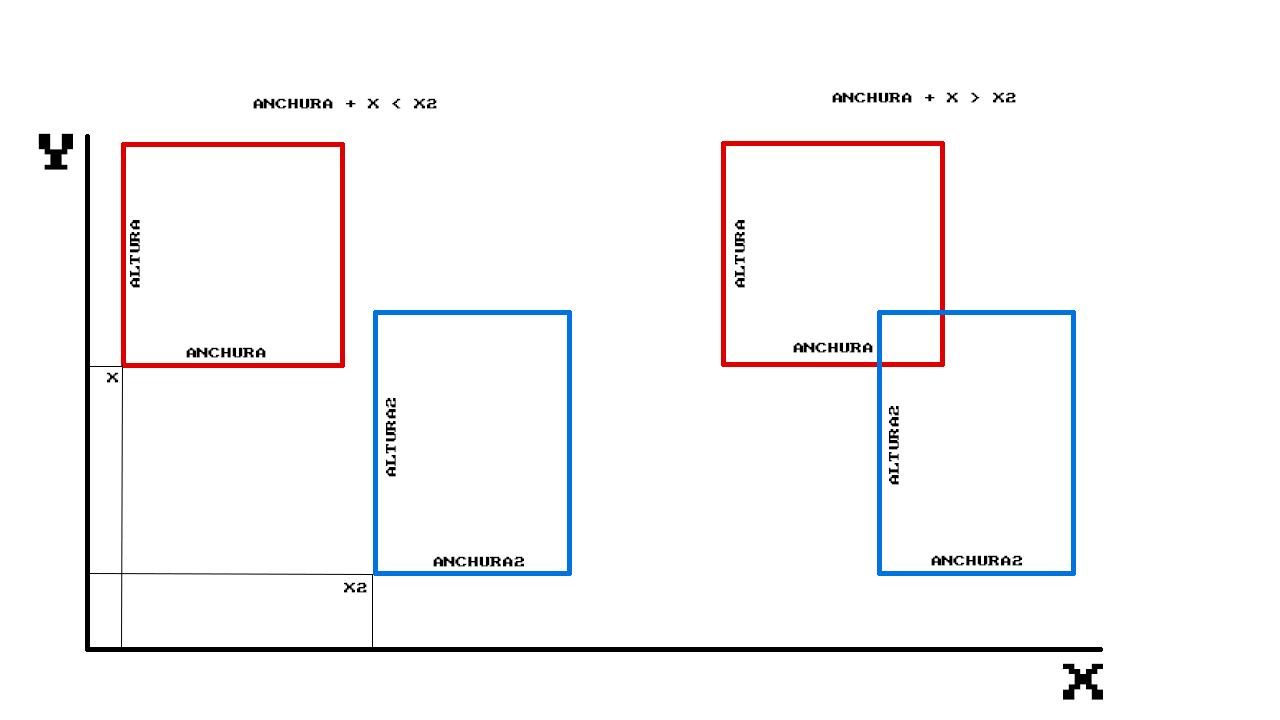
\includegraphics[width=1\textwidth]{include/images/desarrollo/collision_theory.png}
\caption{Colisiones Pixel a Pixel}
\label{figure:collision_theory}
\end{figure}

De hecho, en la GB se puede comprobar las colisiones entre sprites con este método sin problema alguno. ¿Qué ocurre entonces? A pesar de que los sprites tengan coordenadas, el fondo de pantalla o background va por tiles. O dicho de otro modo, \textbf{el fondo no está compuesto por sprites}, los cuales posean coordenadas de pantalla para, posteriormente, nosotros hacer las comprobaciones necesarias.
\\ \\
¿Cómo lo implementamos entonces? Esta es una \textbf{pregunta que muchas personas llegado el momento se plantean constantemente} durante un cierto tiempo. "Dadas las coordenadas de pantalla de nuestro personaje, calculemos en qué tile está situado exactamente al inicio de partida". Esta es la \textbf{primera respuesta alguien se puede dar}. El \textbf{resultado} de ello va a ser \textbf{desastroso}, ya que se necesitan demasiados cálculos (y no solo de 8 bits, sino de 16 bits) para poder lograrlo. Además, el código se hace infinito y muy poco óptimo.
\\ \\
Lo mejor es \textbf{optar por las ideas más sencillas} (y con más sentido), por ejemplo, \textbf{guardar desde un principio el tile} (precalculado) en el que se encuentra el personaje. Digamos que si su posición en coordenadas es la (80,80), siendo el valor del scroll (0,0), el tile del personaje es el (9,9). \textbf{Los cálculos son sencillos}: se dividen las coordenadas del personaje entre 8 (tamaño de un tile) y le resto 1. Esta última operación es por como he diseñado el juego y por comodidad, ya que todos los bloques son de 2x2 tiles, menos los límites de pantalla que los tengo diseñados de 1x1 tiles.

\begin{figure}[h]
\centering
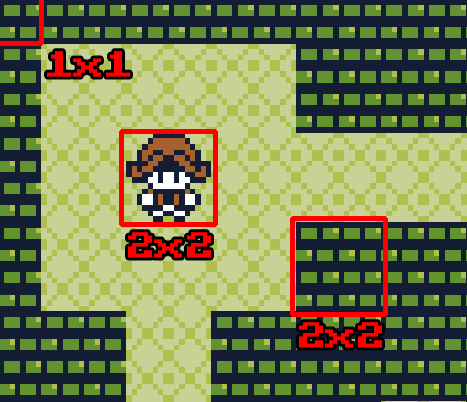
\includegraphics[width=0.5\textwidth]{include/images/desarrollo/tiles_width.png}
\caption{Tamaño de Bloques en el Juego}
\label{figure:tiles_width}
\end{figure}

A continuación, lo que debemos hacer es un poco más complejo: comprobar el tile al que nos vamos a mover, dependiendo de la dirección que nos indique el PAD. Lo primero a encontrar es la dirección de memoria de vídeo que nos indican los tiles del personaje. Empezando desde la dirección inicial de la pantalla, se le sumará en bucle en valor 32 hasta que el tile Y del jugador se quede a 0 (obviamente, sin borrar el dato inicial). Cuando esto último ocurra, se le suma directamente el tile X, y de esta manera ya habremos conseguido la posición de memoria en la que se encuentra el personaje.

\begin{lstlisting}[caption={Encontrar dirección de memoria del tile de personaje}, label={code:check_tile}]
CM_CHECK_TILE:

	ld 	 hl, _SCRN0 				;32x32 tiles
	ld 	 e, 32
	ld 	 d, 0
	ld 	 b, 0
	ld 	 a, [_TILE_Y] 				

cnt_yloop:

	;Moverse primero en el eje Y --> añadir 32
	add  hl, de
	inc  b
	cp   b
	jr 	 nz, cnt_yloop
	
	;Moverse en el eje X --> añadir 1
	ld 	 a, [_TILE_X]
	ld 	 e, a
	add  hl, de
	ret
\end{lstlisting}

¿Queremos comprobar el tile izquierdo? Le restamos 1 a esa dirección. ¿Queremos comprobar el tile de abajo? Le sumamos 32.
\\ \\
Por último se deberá de comprobar si podemos mover los sprites a ese tile. Lo que haremos será implementar un \textbf{listado de bytes} (seguidos, uno tras otro) de los \textbf{números de tile a los que el personaje se puede mover}, y comprobar si coincide con alguno de esos. En caso contrario, denegaremos el movimiento.
\\ \\
Como podemos observar, el proceso es algo más complejo que las dos comprobaciones que se hacen habitualmente en cualquier juego 2D, pero no por ello imposible. \textbf{Lo único que hay que tener en cuenta en todo momento es que el bus de datos no se corrompa}. Es decir, que cuando vayamos a comprobar el valor de la susodicha dirección de vídeo, el LCD se encuentre en V-Blank o H-Blank. Si necesitas algo más de información ve al apartado \textbf{\hyperref[anexo_gpu]{9.6}}.

\subsection{Enemigos}

La inteligencia artificial de los enemigos en esta iteración se puede describir como un 'pilla-pilla', sin mucho más. De forma general, en la mayor parte de los juegos \textit{RPG} el comportamiento de los enemigos es ese, con añadidos como el sentido de visión o las diferentes estadísticas.
\\ \\
Lo primero que vamos a hacer es \textbf{diseñar unos sprites sencillos} del típico esqueleto que te encuentras en cualquier juego \textit{RPG}. La única condición que vamos a tener es que el sprite debe ser de 2x2 tiles, para que luego no hayan problemas con los cálculos de colisiones.

\clearpage

\begin{figure}[h]
\centering
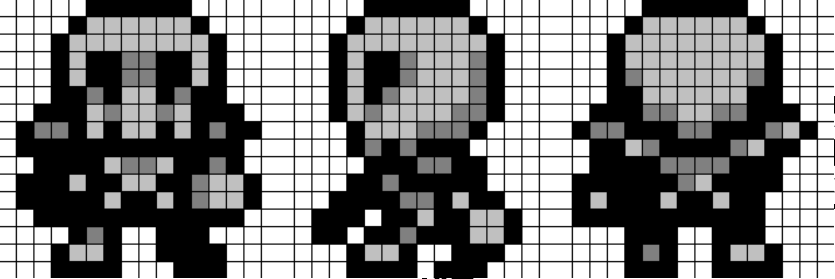
\includegraphics[width=0.7\textwidth]{include/images/desarrollo/enemy_sprite.png}
\caption{Primer Diseño de Enemigo}
\label{figure:enemy_sprite}
\end{figure}

Ahora que tenemos un sprite lo siguiente es conseguir que se mueva por la pantalla. "¿En qué dirección?", es la pregunta que nos debemos hacer. Aunque la IA persiga al jugador, \textbf{si no le controlamos las colisiones va a poder moverse por donde más le convenga}. Dicho pues, el primer paso va a ser calcularle las colisiones, exactamente \textbf{igual que se ha explicado con el jugador}. La única \textbf{diferencia} es que en vez de coger el valor de los inputs, debemos \textbf{usar el valor pasado por parámetro} al cual la entidad intente moverse.

\begin{lstlisting}[caption={Comprobación de Colisiones del Enemigo}, label={code:check_tile_en}]
CM_CHECK_NEXT_TILE_EN:

	ld 	 c, a
	call CM_CHECK_TILE 		; Devuelve en HL la dirección de memoria del tile.

	ld 	 a, c
	or 	 a
	jr 	 z, cnt_top 		; Move enemy up
	dec  a
	jr 	 z, cnt_bot 		; Move enemy down
	dec  a
	jr 	 z, cnt_left 		; Move enemy left
	jr 	 cnt_right 			; Move enemy right
\end{lstlisting}

¿Qué input le pasamos? Es lo "único" que nos queda por calcular. Realmente necesitaremos programar varias funciones que calculen la dirección a seguir de manera distinta. El mayor problema de la GB es el del \textbf{tiempo}, en el sentido de que si nos salimos del intervalo V-Blank no vamos a poder continuar comprobando el valor de las casillas. Y ,a diferencia del jugador, en este caso no vamos a comprobar una dirección en un mismo ciclo de cómputo: \textbf{en el peor de los casos vamos a querer comprobar las cuatro direcciones posibles}.
\\ \\
Así pues, vamos a tener que simplificar lo máximo posible todos los cálculos, dejándolo, por ejemplo, de la siguiente manera:

\begin{itemize}
	\item \textbf{1:} Comparamos coordenadas Y. Si son idénticas, pasamos directamente a comprobar las coordenadas X.
	\item \textbf{2:} Si las coordenadas Y eran distintas, miramos si el tile del enemigo es mayor que la del jugador. Si lo es, intentamos moverlo hacia arriba, si no lo es, hacia abajo.
	\item \textbf{3:} Si no hemos podido moverlo en Y por la condición del punto 1 o por colisiones en el punto 2, comparamos las coordenadas X. Si hemos podido moverlo, saltamos al punto 6.
	\item \textbf{4:} Si la coordenada X del enemigo es mayor, intentamos moverlo hacia la izquierda. En caso contrario, hacia la derecha.
	\item \textbf{5:} Si se han encontrado colisiones, salimos de la función y no actualizamos el movimiento del enemigo.
	\item \textbf{6:} Guardamos en la variable del enemigo la dirección resultante para, en el siguiente ciclo, iniciar el movimiento.
\end{itemize}

Ya tenemos el movimiento terminado. ¿Qué nos queda? Obviamente, \textbf{conseguir que ataque al jugador y le haga daño}. Esto es muy simple: simplemente comprobamos, previo a realizar los pasos expuestos, si el jugador está en una casilla adyacente. En caso de estarlo, \textbf{iniciamos una animación de ataque y al terminar le restamos vida al jugador}.

\begin{figure}[h]
\centering
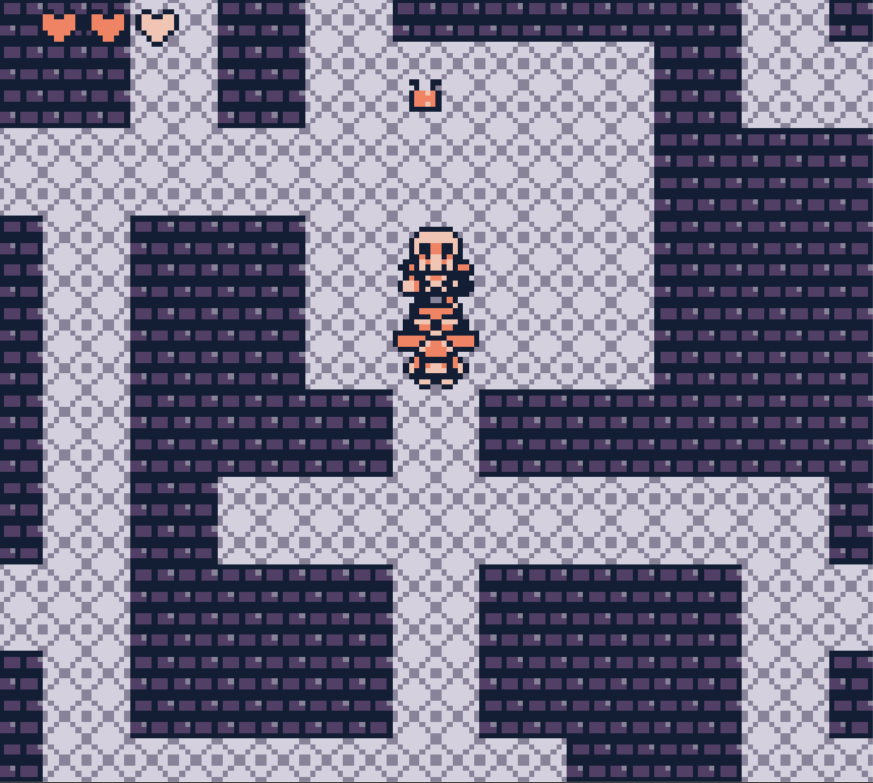
\includegraphics[width=0.5\textwidth]{include/images/desarrollo/enemy_attack.png}
\caption{Ataque del Enemigo}
\label{figure:enemy_attack}
\end{figure}

\subsection{Paletas}

Este es un tema que muchos comenzamos a estudiar por mera curiosidad. En nuestra infancia siempre nos hemos preguntado por qué algunos juegos se veían en blanco y negro en la GB, mientras que, si los ponías en la GBC, repentinamente obtenían color. Y cómo no, esto sucedía solamente en casos específicos como el Pokémon Plata/Oro.
\\ \\
Esto se debía a que, según qué desarrolladora, \textbf{se molestaron en programar en el susodicho juego las paletas de colores} para que fuese más vistoso jugarlo en la GBC.

\clearpage

\begin{figure}[h]
\centering
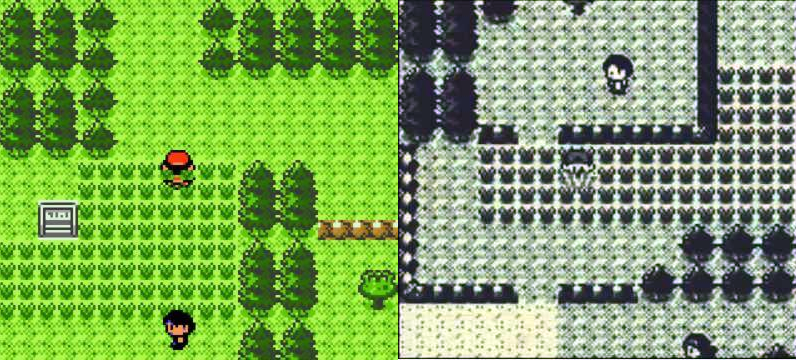
\includegraphics[width=0.8\textwidth]{include/images/desarrollo/paletas_pokemon.png}
\caption{Pokémon Rojo/Azul en GBC y GB}
\label{figure:poke_palette}
\end{figure}

A día de hoy aún es complicado encontrar información al respecto para poder conseguir este efecto. Por suerte, \textbf{el manual oficial de la CPU de \textit{Nintendo} describe en detalle el proceso a seguir}. No incluye ningún tipo de ejemplo, pero ya es más que suficiente.
\\ \\
Lo primero que debemos hacer es comprobar qué Game Boy está utilizando el jugador. Esta parte es bastante sencilla, ya que \textbf{el hardware nos inserta en el registro 'a' un booleano que nos lo indica}. Con este valor ya podemos pasar a insertar las paletas.
\\ \\
Empecemos por el caso de la GB, el cual es el más sencillo de implementar:
	
\begin{lstlisting}[caption={Paleta para la GB}, label={code:palette_GB}]
	BCK_PALETTE 	EQU %11100100
	SPR_PALETTE 	EQU %11100010
	GBC 			EQU $11

	[...]
	
	cp   GBC
	jr   z, .gbc

	ld   a, BCK_PALETTE 	;cargar dirección de memoria de la paleta en a
	ld   [rBGP],  a  		;paleta de fondo
	ld   a, SPR_PALETTE
	ld   [rOBP0], a  		;paleta para sprites
\end{lstlisting}

Como podéis apreciar, lo único que hacemos es \textbf{insertar un byte en los registros rBGP y ROBP0 para la paleta de fondo y de sprites, respectivamente}. La GB interpreta el valor que le hemos introducido como grupos de 2 bits, siendo 00 el blanco y 11 el negro. \textbf{Los bytes en el registro indican el rango del color más oscuro al más claro}. \textbf{El primer byte de la paleta de sprites}, independientemente del valor que le demos, \textbf{va a ser transparente}.
\\ \\
Por otro lado, en el caso de la GBC, la cosa se complica. Nos tenemos que hacer dos funciones, una para la paleta de fondo y otra para los sprites. \textbf{La GB posee dos direcciones de memoria que funcionan como si de un array se tratase}. Tenemos por un lado el registro \textbf{\$FF68 o rBCPS} que funciona como \textbf{índice}, mientras que \textbf{\$FF69 o rBCPD} son las \textbf{posiciones donde meter los valores correspondientes}. Dejar claro que estas direcciones de memoria mencionadas son las pertinentes a la paleta de fondo.

\begin{lstlisting}[caption={Paleta para la GBC}, label={code:palette_GBC}]
dungeon_palette:
DB $32, $AF, $0F, $0F, $07, $06, $02, $10

Set_Dungeon_Palette:

	ld 	 b, 4
	ld 	 hl, dungeon_palette

	xor  a
	set  7, a 			
	ld 	 [rBCPS], a 		;Auto Increment. This is a Write-Specification register.

set_dbp:

	ld 	 a, [hl+]
	ld 	 [rBCPD], a 		;This is a Write-Data register.
	ld 	 a, [hl+]
	ld 	 [rBCPD], a

	dec  b
	jr   nz, set_dbp

	ret
\end{lstlisting}

En este caso disponemos de 16 bytes que representan los 4 colores. Descontando el byte mayor (5 bytes para cada canal de color), tenemos \textbf{$2^{15}$ = 32768 colores distintos}. Los primeros 5 bytes son para el canal rojo, los siguientes para el verde, y los más altos para el azul.
\\ \\
En cualquier caso, \textbf{si necesitas más información} al respecto visita el \textbf{apartado \textbf{\hyperref[anexo:lcd_color]{9.6.3}}} del anexo.

\clearpage

\subsection{Interrupción V-Blank}

Leyendo la documentación oficial de la CPU, podemos llegar a un interesante apartado en el que explican \textbf{cómo optimizar las comprobaciones de llegada al rango V-Blank}.
\\ \\
Hasta ahora, lo único que habíamos llegado a ver era el siguiente ejemplo:

\begin{lstlisting}[caption={Espera al rango V-Blank: Método 1}, label={code:vblank1}]
WAIT_VBLANK:
	ld	a,[rLY]				;get current scanline
	cp	145					;Are we in v-blank yet?
	jr	nz,WAIT_VBLANK		;if A-91 != 0 then loop
\end{lstlisting}

Es un método bastante sencillo que nos puede ayudar en una primera instancia para esperar al rango V-Blank. Sin embargo, \textbf{es una mala práctica} ya que \textbf{consume mucha más batería} de la consola que haciéndolo de la manera que veremos a continuación. Además, sin ir más lejos, la comprobación la realizan (por lo general) con el valor 145, cuando el rango de V-Blank comienza en el 144 (por minúsculo que parezca, ya es un microsegundo que perdemos por ciclo de juego).
\\ \\
¿Cómo recomiendan hacer estas comprobaciones? Mediante el \textbf{uso de su interrupción} (puedes ver \textbf{más información} en el \textbf{apartado del anexo \textbf{\hyperref[anexo:interruptions]{9.5}}}).
\\ \\
La idea es simple: \textbf{cuando queramos esperar al V-Blank, hacemos un "halt"} para dejar la consola en stand-by, a la espera de que se produzca cualquier interrupción. La cuestión es que no queremos que eso ocurra, \textbf{solo queremos que salga de la espera cuando la interrupción sea la apropiada (la del V-Blank)}. Dicho pues, lo primero que hacemos en nuestra configuración es activar solamente la ya mencionada:

\begin{lstlisting}[caption={Activar Interrupción V-Blank}, label={code:enable_vblank}]
IEF_VBLANK 	EQU %00000001

	[...]

;enable vblank interrupt
 	ei
	ld   a,IEF_VBLANK
	ld   [rIE],a
\end{lstlisting}

Al llegar al vector \$40, vamos a \textbf{insertar un 1 en una variable global} que nos indica cuándo hemos accedido a la interrupción. Esta variable global \textbf{la iremos comprobando en la función de espera}:

\begin{lstlisting}[caption={Espera al Rango V-Blank: Método 2}, label={code:vblank2}]
RS_WAIT_VBLANK:

  	halt
  	nop
  	
  	ld 	 a,[vblank_flag]
  	or 	 a
  	
  	jr 	 z, RS_WAIT_VBLANK

  	xor  a
  	ld   [vblank_flag],a

	ret
\end{lstlisting}

De esta manera, \textbf{no optimizamos en bytes de código}, pero \textbf{la batería} de la GB del jugador \textbf{va a durar mucho más} (puede llegar a extender su vida en un 50\%).

\subsection{Acceso Directo a Memoria}

\textbf{Optimizar el código siempre es una buena práctica} y más en este tipo de proyectos en los que disponemos de recursos tan limitados. Aquí es donde el proceso de \textbf{Acceso Directo a Memoria o Direct Memory Access (DMA)} entra en juego.
\\ \\
Sabemos que para crear un sprite necesitamos variables guardadas en la OAM, las cuales más tarde la consola interpreta y muestra. El problema con el que nos vamos a topar en cuanto tengamos distintas entidades actualizándose simultáneamente es el de que, para hacerlo, necesitamos estar dentro del rango V-Blank (ya que, de otra forma, la memoria de vídeo es inaccesible). Si además de esto, queremos actualizar la lógica de nuestro juego en este período corto de tiempo, el problema obtiene un efecto \textit{bola de nieve}.
\\ \\
\textbf{El DMA nos ahorra todo este trabajo}, ya que es capaz de enviar bytes de información desde la ROM/RAM a la OAM cada cierto tiempo. Remarcar antes que nada que esta transferencia de datos \textbf{dura apenas 160 ciclos}, lo cual es un tiempo diminuto.
\\ \\
Lo primero que deberemos hacer es \textbf{reservar e inicializar un bloque de memoria RAM}. Concretamente, este bloque debe debe ocupar 160 bytes, ya que el proceso transfiere un byte de RAM a OAM por ciclo. Es recomendable reservarlos comenzando en la posición \$C000.

\begin{lstlisting}[caption={Reserva de Memoria para DMA}, label={code:dma_space}]
SECTION "DMA_VARS", WRAM0[$C000]

;PLAYER SPRITES

_SPR0_Y: DS 1
_SPR0_X: DS 1
_SPR0_NUM: DS 1
_SPR0_ATT: DS 1

[...]

free_space: DS 108

\end{lstlisting}
\clearpage
A continuación, vamos a ver el código necesario para que el DMA ocurra:
\\ \\
Existe un \textbf{registro especial (\$FF46)} en el que tendremos que indicar la dirección en la que empiezan los datos a transferir. Como solamente son dos bytes, por defecto los bajos serán 00. Una vez metamos el valor en el registro, el DMA comenzará inmediatamente, por lo que tendremos que mantenernos dentro de un bucle a la espera de que termine.

\begin{lstlisting}[caption={Inicio del proceso DMA}, label={code:dma_wait}]
  ld      a, $C0 			;Carga la dirección de memoria $C000
  ld      [$FF46], a

  ld      a, $28 			;Espera 160 microsegundos
.loop:
  dec     a
  jr      nz, .loop
  ret
\end{lstlisting}

El problema es que \textbf{mientras el proceso de DMA ocurre, el hardware solo puede acceder a HRAM}. Si implementásemos la función tal y como la he descrito en el código de arriba, se almacenaría en ROM, por lo que \textbf{no llegaría a ejecutarse nunca}.
\\ \\
Lo que vamos a hacer es \textbf{guardar todo ese código en la dirección \$FF80}, la cual es HRAM, de la siguiente manera:

\begin{lstlisting}[caption={Copiado de Proceso DMA}, label={code:dma_copy1}]
	ld  de,$FF80
	rst $28
	DB  $00,$0D

  	DB  $F5, $3E, $C0, $EA, $46, $FF, $3E, $28, $3D, $20, $FD, $F1, $D9
  	ret
\end{lstlisting}

Como ves, lo primero que hacemos es cargar en los registros 'DE' la dirección ya mencionada. Lo siguiente es \textbf{provocar un reset de la consola}, lo cual llamará a la interrupción correspondiente (y ahí meteremos el código). ¿Por qué no hacer una función y llamarla con "call"? Porque el opcode "rst" ocupa 1 byte, lo que equivale a ser más rápido.
\\ \\
Los siguientes 2 bytes los utilizaremos de contador para indicar cuánta información copiar. Y por último tenemos 13 bytes que no son, ni más ni menos, que el código de \textbf{\hyperref[code:dma_wait]{Inicio del proceso DMA}}. A la hora de copiarlo es más sencillo disponer de una tira de bytes a tener lenguaje ensamblador.
\\ \\
Lo único que nos falta es escribir nuestra rutina de copiado en la interrupción ya mencionada, la cual \textbf{tiene como dirección de memoria \$0028}:

\clearpage

\begin{lstlisting}[caption={Rutina de Copiado en Interrupción para DMA}, label={code:dma_copy2}]
SECTION "Reset Table",ROM0[$28]
COPY_DMA_DATA:
	pop hl 					;here we get the return address onto hl. It is the top of the stack
	push bc 				;we save the value of bc just in case it has something important

	; here we get the number of bytes to copy
  	; hl contains the address of the bytes following the "rst $28" call

	ld  a,[hli]
	ld  b,a
	ld  a,[hli]
	ld  c,a

	;now bc contains the total bytes to copy ($000D)
	;and hl points to the first byte of our assembled subroutine (which is $F5)

COPY_DMA_DATA_LOOP:

	ld  a,[hli] 			;save the data of hl in a and increase it
	ld  [de],a 		 		;save the data of  a in de (FF80)
	inc de 					;increase the memory address of the destination
	dec bc 					;decrease the byte counter
	ld  a, b 				
	or  c
	jr  nz, COPY_DMA_DATA_LOOP
	pop bc 					;restore the initial value of bc
	push hl 				;push on to the stack the memory address which is the ret of the DMA_COPY function
	reti					;return to the top of the stack memory address
\end{lstlisting}

Paso a paso: hacemos un pop a la pila para obtener el valor que tenía de vuelta, el cual es el primer byte \$00 de nuestro \hyperref[code:dma_copy1]{\textbf{Copiado de Proceso DMA}}. De paso, guardamos en la pila el valor que tuviese los registros 'BC' por si hubiese información importante.
\\ \\
Nos guardamos en 'BC' los dos bytes que nos indicaban el tamaño de datos a copiar para usarlo de contador, y comenzamos a meter en las direcciones de los registros 'de' los valores de 'HL' hasta que 'BC' llegue a 0. Una vez terminado, devolvemos a 'BC' su valor inicial sacándolo de la pila y hacemos un push de la dirección de memoria actual en 'HL' para, a continuación, volver con un "reti".
\\ \\
Y para terminar, lo único que tenemos que hacer es, en nuestro bucle principal del juego, hacer un call a la dirección de HRAM para dejar paso al proceso DMA.

\subsection{Ventanas}

Las ventanas de HUD se han intentado implementar en esta iteración. Pese a que se ha implementado tanto la del menú general como la de diálogo (sin texto), \textbf{se ha llegado a la conclusión de que hay que rehacerlo}. Aún así, no está de más dejar por escrito el proceso que se ha seguido:

\begin{figure}[h]
\centering
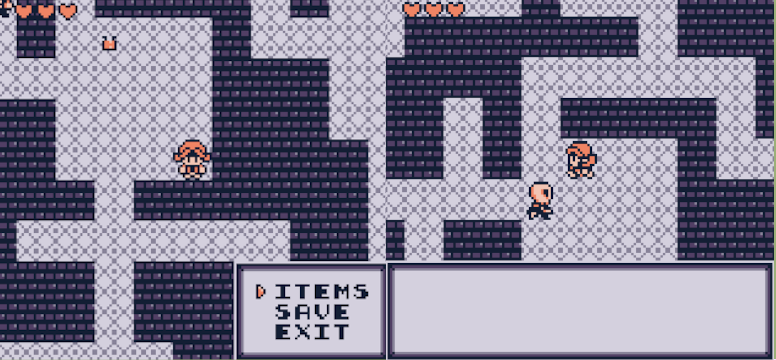
\includegraphics[width=0.6\textwidth]{include/images/desarrollo/hud1.png}
\caption{Primera Iteración del HUD}
\label{figure:hud1}
\end{figure}

Lo primero que hacemos, al igual que con los mapas de fondo, es \textbf{hacernos nuestros propios tilemaps} con las ventanas que queramos mostrar. El problema con el que nos vamos a encontrar es el del intervalo V-Blank y su pequeño lapso de tiempo.
\\ \\
\textbf{Copiar y pegar una tira tan larga de bytes, sin apagar el LCD}, y que no se produzca basura visual, \textbf{es simple y llanamente imposible}. ¿Cómo lo solventamos? Podemos modificar la función de copiado de memoria con el fin de, en vez de copiar un tilemap entero, copiar una porción (usando para ello un contador).
\\ \\
Sin ir más lejos, la función obtiene como input el valor del contador (ancho de la ventana a copiar) y un offset (cuantos bytes quedan hasta llegar a la siguiente línea de pantalla). De esta manera, \textbf{solamente copiamos la cantidad exacta de bytes} que ocupan esa ventana y no malgastamos tiempo.
\\ \\
El \textbf{dónde copiarlo}, sin embargo, no va a ser la misma dirección de memoria que con el mapa de fondo, si no la \textbf{segunda pantalla} (escondida por defecto) de la que dispone la Game Boy, cuyo \textbf{rango va desde la dirección \$9C00} (la cual indicaremos ahora como destino) \textbf{hasta la \$9FFF}.
\\ \\
Para mostrar esta pantalla, deberemos hacer lo siguiente:

\begin{lstlisting}[caption={Encendido de la Segunda Pantalla}, label={code:show_screen}]
SHOW_SCRN1:

	;Encendemos la pantalla LCD
	ld a, [rLCDC]
	or LCDCF_WINON
	ld [rLCDC], a
	
	;La coordenada Y de pantalla será el parámetro B
	ld a, b
	ld [rWY], a

	;La coordenada X de pantalla será el parámetro C
	ld a, c
	ld [rWX], a
	ret
\end{lstlisting}

Como parámetros de entrada necesitaremos las coordenadas X e Y que queremos que tenga la pantalla. Lo que resta es ponerle a la \textbf{dirección de memoria \$FF40 (rLCDC)} el valor \%00100000 (LCDCF\_WINON), que \textbf{especifica el encendido de la segunda pantalla}.
\\ \\
\textbf{El problema} del rango V-Blank, después de todo, \textbf{seguía ocurriendo}, por lo que la única solución que quedaba era apagar y encender la pantalla LCD. Esto provoca que se perciba un \textbf{parpadeo poco agradable a la vista}.

\subsection{Sonido}

Los \textbf{efectos de sonido y la música} en la actualidad son \textbf{esenciales} en un juego. Sin ellos, no solo eres incapaz de producir cualquier estímulo al jugador, si no que no das ningún tipo de \textit{feedback} auditivo sobre lo que está ocurriendo.
\\ \\
Viniendo de sistemas modernos donde simplemente reproducimos un fichero de texto, puede ser un apartado bastante complejo.
\\ \\
En el caso de la GB, dispondremos de \textbf{4 canales por los que ser capaces de emitir sonidos}. El propio hardware se encargará de mezclarlos y dar el output que corresponde. No vamos a verlos en este apartado, si necesitas \textbf{más información} visita el punto del \textbf{anexo \hyperref[anexo:sonido]{9.7}}.
\\ \\
Lo primero que vamos a hacer es \textbf{inicializar los registros de uso general}. Tenemos, por ejemplo, \textbf{rNR52 (\$FF26)}, que activa o desactiva por completo el sistema de audio. 

\begin{lstlisting}[caption={Inicialización Registros de Sonido de Uso General}, label={code:generalregisters}]
        ld              a, %00000111            ; Volumen Máximo del Output 1 y 2.
        ld              [rNR50], a
 
        ld              a, %00000010            ; El Canal 2 solamente saldrá por el Output 2.
        ld              [rNR51], a
        
        ld              a, %10000000
        ld              [rNR52], a 			 	; Encendido del sistema de audio.
\end{lstlisting}

Ahora, por cada ciclo de ejecución, vamos a \textbf{actualizar la "nota"} que nuestro sistema de audio va a hacer sonar. Como estas notas musicales van a estar en la misma octava, longitud, ciclo de trabajo y envolvente, podemos inicializar solamente una vez los registros de uso general en las siguientes direcciones de memoria: rNR21, rNR22 y rNR24. La frecuencia "baja" de nuestra nota va a estar guardada en rNR23. También vamos a disponer de un \textbf{tempo} por el cual podamos \textbf{conseguir distintos ritmos}.

\begin{lstlisting}[caption={Sonido en Canal 2}, label={code:channel2}]
		call 		  Check_Tempo 		; Comprobar que podemos cargar la siguiente nota
		or 	  	  a
		ret 	  	  nz
		call 	 	  Reset_Tempo 		; Reiniciar el contador del tempo		
		
		ld             a, [_NOTA]              ; Cargamos la nota a tocar
        ld              c, a                    
        ld              b, 0 						; BC = Número de nota a tocar
        
        ld              hl, Music_Notes    ; HL = Dirección ROM donde están nuestras notas musicales
        add          hl, bc                  		; ahora tenemos la dirección de la nota a tocar
        ld              a, [hl]                	
        ld              [rNR23], a              ; la escribimos en el registro
 
       call 		   Save_Note  			; Comprobamos si es la última nota musical (de ser así reiniciamos a la primera). En caso contrario cargamos la siguiente.
       
\end{lstlisting}

\subsection{Conclusión}

Como conclusión de esta iteración, comentar que \textbf{se han conseguido con creces todas las tareas propuestas}. Ya disponemos de un prototipo en el cual nos podemos mover, matar, morir, coger un objeto, y escuchar algún que otro sonido. Quedan \textbf{asuntos pendientes} como que el juego sea extremadamente lento, que no podamos tener más de un enemigo, o que para mostrar la ventana de texto tengamos que apagar y encender la pantalla. Sin embargo, puedo decir que \textbf{estoy contento con el resultado obtenido}.

\clearpage

\section{Iteración 2 - Reestructuración y Reimplementación de Código}

Esta iteración se ha basado principalmente en la \textbf{reestructuración del código}, basándose ahora en el modelo \textbf{Entity Component System} (\textbf{ECS}), dejando lo conseguido en la iteración 2 como prototipo del cual poder avanzar, y \textbf{centrándonos en hacer reescalable el código} por medio de la creación de \textbf{arrays de entidades}.

\subsection{Entity Component System}

En el prototipo de la iteración 1 podiamos tener, única y exclusivamente, un enemigo. Además, se hacía cuesta arriba el poder realizar su actualización al mismo tiempo que la del jugador, ya que cada función contenía tanto las decisiones lógicas de la IA como el calculo de colisiones, animaciones, etc. Por ello, a la hora de jugar, se podía ver cómo el enemigo solamente tomaba decisiones en acabar la ronda del jugador, lo que además provocaba una \textbf{experiencia lenta}.

\begin{figure}[h]
\centering
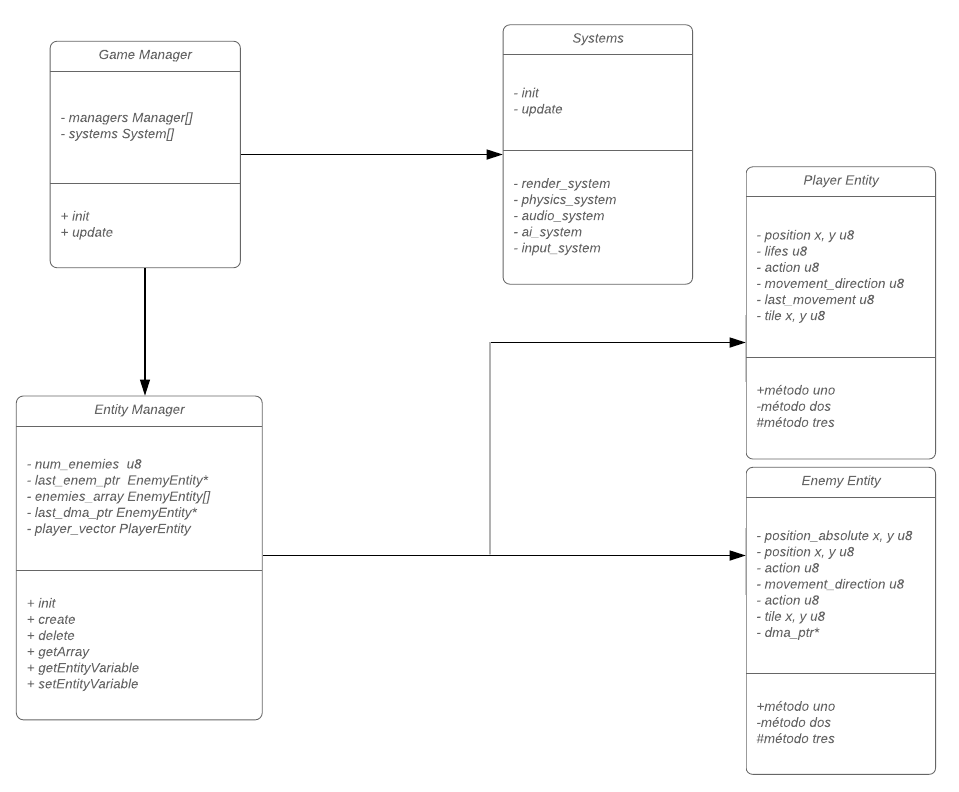
\includegraphics[width=1\textwidth]{include/images/desarrollo/Diagrama.png}
\caption{Diagrama ECS}
\label{figure:ecs}
\end{figure}

Con el modelo ECS, sin embargo, \textbf{podemos independizar todas las tareas en sistemas y manejadores de datos}, con lo que seremos capaces de actualizar todo lo que contenían antes tanto el jugador como el enemigo, en un preciso instante de tiempo. Es decir, podemos actualizar la inteligencia artificial de los enemigos por un lado, para luego actualizar el renderizado, y más tarde pasar a las físicas de todas las entidades.
\\ \\
Ya no solo nos ayuda a corregir estos problemas, sino que además habremos conseguido tener el código mucho más legible y ordenado de lo que en un principio estaba. \textbf{Las tareas se han conseguido independizar las unas de las otras y centralizar aquellas operaciones que crean, modifican o destruyen datos en los manejadores}. \\

\subsection{Array de Entidades}

Para la creación y manejo de un array veremos que el proceso un tanto complejo: \\

A la hora de crear el array, debemos que \textbf{tener claras dos cosas: cuántas entidades queremos que hayan al mismo tiempo y cuántos datos va a contener cada entidad}. Una vez hecho esto, simplemente le tenemos que decir al compilador que nos reserve un \textbf{Número de entidades * Tamaño de Entidad}. También querremos un \textbf{puntero a la última posición en la que podemos crear un enemigo}, la cual es simplemente la etiqueta con la que accederemos al primer valor y el que va a ir incrementando cada vez que creemos otra entidad.

\begin{lstlisting}[caption={Reserva Memoria}, label={code:memory}]

    ;==============================================================
    ; Compilation time constants
    ;==============================================================

    enemy_size      = 9
    max_entities 	= 3

    SECTION "Entities_Data", WRAM0[$C000]

    ; Each sprite needs 4 bytes, that means we can store 160/4 = 40 sprites
    dma_enemies:    DS 64 	; Each enenemy consists of 4 sprites

    num_enemies: 	DS 1

    last_dma_ptr:   DS 2
    last_enem_ptr: 	DS 2

    player_vector:  DS player_size
    enemie_array: 	DS enemy_size*max_entities
    block_array: 	DS block_size*max_items

\end{lstlisting}

\clearpage

Sin embargo, para el caso de la Game Boy vamos a tener que crear \textbf{dos arrays distintos}. \textbf{Uno al cual pueda acceder el DMA} (el cual contendrá solamente datos para almacenar en la OAM) y un array en el cual poder almacenar los \textbf{datos restantes como la acción que tiene que hacer o la dirección de movimiento}.
\\
Por ello, tanto a la hora de crear como destruir una entidad, hemos tenido que trabajar con dos arrays distintos, los cuales contienen distintos tipos de datos, y solamente con instrucciones de 8 bits (esto en \textit{Amstrad} es bastante más sencillo al disponer del registro 'IX').
\\ \\
Para \textbf{crear una entidad} deberemos que \textbf{seguir los siguientes pasos}: coger la dirección del último puntero, leer y copiar los datos desde ROM (con nuestra función de copiado de memoria), poner la siguiente posición como último puntero en la que podemos crear una entidad y aumentar el número de entidades del que disponemos.
\\
En el caso de este proyecto, hemos realizado algo más complejo (y no por ello mejor). Primero, obtenemos el puntero del cual tendríamos que copiar datos por parámetro. Estos datos eran las \textbf{posiciones absolutas} (recordemos que los enemigos tienen dos posiciones, una de pantalla y otra de tiles), el número de tile que va a tener el primer sprite de cuatro (arriba a la izquierda), vidas, posición precalculada de tiles, dirección de movimiento y acción. 
\\ \\
Con los tres primeros datos lo que tengo que hacer es rellenar los datos pertenecientes al array del DMA. Es decir, debo hacer los cálculos apropiados para, a partir de las posiciones absolutas que me dan (recordemos que cada entidad son cuatro sprites juntos), calcular las posiciones de pantalla. También, con el número de tile, debemos incrementarlo y ponérselo al sprite que toque. Esto se traduce en un trozo de código poco legible y que a la larga puede suponer problemas, pero de momento nos sirve.
\\ \\
Con el puntero de la última posición donde podemos crear un enemigo, y con el dato de cuánto ocupa cada entidad (que en este caso sería Tamaño de Entidad-2, ya que los dos primeros datos se guardan junto a los cálculos previos), llamamos a una función de copiado de memoria, el cual ya tenía el origen (el primer puntero pasado por parámetro), destino y tamaño de datos a copiar. Solo queda actualizar ambos punteros de última entidad, aumentar el número de enemigos y listo, ya tenemos una entidad creada.
\\ \\
Para el borrado fue algo más sencillo, ya que simplemente modificamos el tamaño de las entidades y les añadimos un puntero a la posición que les toque en el array de DMA. Con el puntero del array de entidades pasado por parámetro, nos vamos al puntero del DMA de esa entidad. \textbf{Cada entidad en DMA ocupa 16 bytes (4 bytes por sprite)}, con lo que ya sabemos el tamaño de datos con el que vamos a lidiar. Ahora obtenemos el puntero al último enemigo del array de DMA y, nuevamente, copiamos y pegamos datos de uno al otro. En este caso tendremos que asegurarnos de que los datos de la última entidad se borren ya que lo que se quede en este array se va a visualizar por pantalla. Actualizamos el último puntero de DMA a la entidad copiada y una cosa menos de la que preocuparse.
\\ \\
Volviendo al otro array, la idea es exactamente la misma, con la diferencia de que no hace falta poner a 0 todos los bytes de la entidad eliminada. Simplemente con decrementar el número de entidades, esos datos ya no se van a usar.
\clearpage
Y por último, para poder iterar sobre todos los enemigos y actualizarlos de forma continua, hemos creado una pequeña función que devuelve los punteros de ambos arrays y el número de enemigos que tenemos en ese preciso instante. Simplemente, al terminar de actualizar una entidad, sumamos al puntero el tamaño de la entidad para actualizar la siguiente en un bucle.

\begin{lstlisting}[caption={Get Enemies Array}, label={code:enearray}]
    EM_GET_ENEMIES_ARRAY:
        ld 	 a, [num_enemies]
        ld 	 hl, enemie_array
        ld   de, dma_enemies
        ret

\end{lstlisting}

\subsection{Conclusión}

Si bien parece que, más que avanzar en esta iteración, lo que hayamos hecho haya sido retroceder, creo que era un \textbf{trabajo completamente necesario}. Este sistema de entidades además de facilitar la generación de enemigos, va a ayudar también con los objetos, elementos de HUD, creación de distintos niveles, etc. Lo que debo hacer en la siguiente iteración es \textbf{intentar aprovechar al máximo el tiempo} del que dispongo para que los resultados se hagan visibles.

\clearpage

\section{Iteración 3 - Elementos para un Mínimo Producto Viable}

En esta tercera iteración se han \textbf{seguido añadiendo elementos que ya estaban en el primer prototipo} de finales de iteración 1, pero que tocaban rehacer desde cero porque no eran reescalables.

\subsection{HUD}

Un \textbf{elemento imprescindible} en cualquier videojuego: \textbf{matar y que te maten}. Y para hacer saber cuánto le falta al jugador para morir, lo mejor es una barra de vida a modo de HUD.
\\ \\
En este caso lo que hemos decidido ha sido cambiar los sprites de corazones que tenía al principio por una \textbf{barra} con la que poder representar \textbf{mayores rangos numéricos} y que, claro está, sean intuitivos para el jugador. Los corazones lo que le indicaban era más bien que tenía un máximo de 6 puntos de vida y nada más. En este tipo de juegos, el personaje va ganando \textit{stats} o estafísticas conforme sube de nivel, entre los que destaca el aumento de este último mencionado.

\begin{figure}[h]
\centering
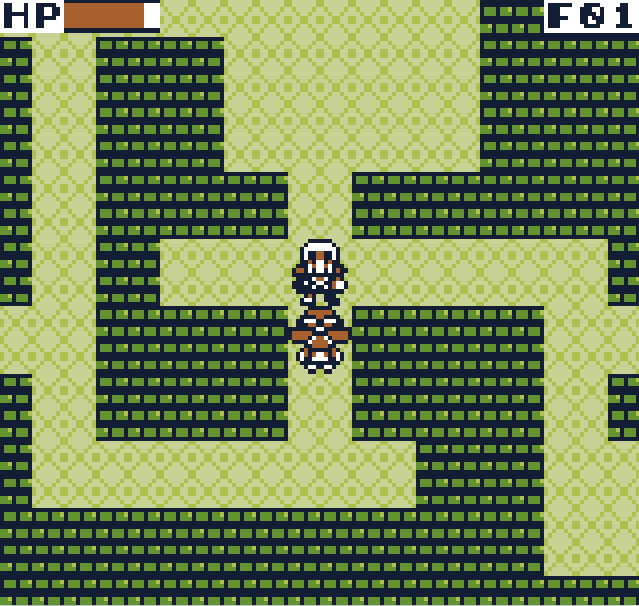
\includegraphics[width=0.5\textwidth]{include/images/desarrollo/lifebar.png}
\caption{Barra de Vida}
\label{figure:lifebar}
\end{figure}

En temas de cómo se muestran los sprites: simplemente son \textbf{variables que almacenamos en la memoria del DMA}. No necesitamos ningún dato en ROM al respecto. Y tampoco tendremos que actualizar la posición absoluta, ya que al ser elementos del HUD \textbf{nos interesa que estén siempre visibles en pantalla}.
\\ \\
La actualización de la barra de vida es sencilla: en la inteligencia artificial de nuestro enemigo, comprobaremos primero si el jugador está en un tile contiguo. En el caso de que lo esté, decrementaremos la vida del jugador (de momento lo haremos en un valor fijo, la idea es que puedan darse golpes críticos o varíe en función de la cantidad de daño), y seguido comprobaremos en qué rango de valores se encuentra nuestro personaje. Esto lo hacemos en divisiones de 6, para poder tener tanto los rangos de los 3 tiles llenos (máxima vida) como vacíos (muerto).
\\ \\
Computacionalmente hablando, no hace falta realizar divisiones en tiempo real para ello, simplemente asignamos de cuánto a cuánto va cada rango, y al valor mínimo de cada uno le restamos la vida actual. \textbf{Si la operación nos genera un acarreo o cero, significa que estamos justo ahí}.

\begin{lstlisting}[caption={Rangos de Vida}, label={code:ranges}]
	; Ranges are: 42-35 | 34 - 28 | 27 - 21 | 20 - 14 | 13 - 7 | 6 - 1 | 0

	ld 	 a, 35
	sub  b 									; This take-away generates carry if we are above the range.
	jr 	 c, vida_completa

	ld 	 a, 28
	sub  b
	jr 	 c, dosenteros_unomitad

	[...]
\end{lstlisting}

También hemos aprovechado para añadir en la esquina derecha superior el \textbf{indicador del piso} en el que nos encontramos. Conforme vayamos avanzando por las mazmorras, el contador irá aumentando.

\subsection{Animaciones}

En todo videojuego son necesarias las animaciones. En el caso de no haberlas, hoy en día la primera reacción del jugador va a ser dejarlo completamente de lado sin pensárselo dos veces.
\\ \\
Si bien en el prototipo que se realizó en la iteración 1 contenía ya un enemigo completamente animado, nos sucede (una vez más) que toca rehacer todo de cero porque el código no se podía reescalar.
\\ \\
Vamos a intentar \textbf{optimizar lo máximo posible} (al menos, dentro de lo que mi conocimiento actual me permite). Lo fácil para hacer animaciones siempre es cambiar el sprite, cada cierto tiempo, sin complicarse mucho más. El problema es que la Game Boy dispone un \textbf{espacio muy limitado de tiles} que podamos usar de forma simultánea, por lo que cuantos menos usemos, mejor.
\clearpage
Dicho pues, el enemigo solamente tiene \textbf{4 sprites}. Y efectivamente, el enemigo se nos puede quedar totalmente animado con solamente esos sprites. Vamos a ver cómo es esto posible:

\begin{figure}[h]
\centering
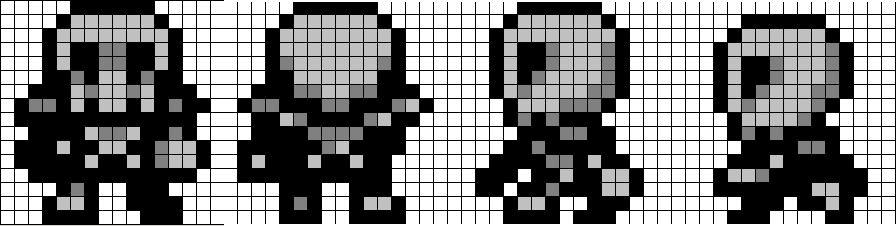
\includegraphics[width=0.5\textwidth]{include/images/desarrollo/animation.png}
\caption{Sprites Enemigo}
\label{figure:animation}
\end{figure}

Ya se ha mostrado con anterioridad estos sprites, pero no está de más recordar cómo son. Si nos fijamos en el primer y segundo sprite, comenzando por la izquierda, podrás darte cuenta de la siguiente particularidad: tienen una pierna hacia delante y otra hacia atrás. Lo mismo ocurre con los brazos. Esto lo hemos hecho a propósito para que pudiésemos crear una animación simplemente \textbf{invirtiendo los sprites}.
\\ \\
En el caso del \textbf{movimiento lateral} ya sí que no nos queda otra que \textbf{hacer uso de dos sprites}, e ir cambiándolos según pase un tiempo. Sin embargo, para el movimiento \textbf{lateral derecho}, lo que haremos será, de la misma manera, \textbf{invertirlos}.
\\ \\
Hacer esto en la GameBoy no tiene mucha complejidad (más allá de gestionarlo de forma correcta). Como ya hemos visto, los sprites en la memoria de vídeo (OAM) constan de \textbf{cuatro valores}: posiciones X e Y, número de tile a usar, y un atributo. Hasta ahora este último siempre lo hemos dejado a 0. Pues bien, toca pasar a manejarlos si queremos tener \textbf{animaciones optimizadas} (en cuanto a memoria de tiles, pues el código para ello nos va a ocupar algo más en ROM).
\\ \\
Principalmente vamos a usar \textbf{dos atributos distintos}, uno para los sprites de arriba, izquierda y abajo, y otro para la derecha (que será el que nos invierta el sprite).

\begin{lstlisting}[caption={Atributos de Sprites}, label={code:attributes}]
RIGHT_ATTRIBUTE EQU %00100000
LEFT_ATTRIBUTE  EQU %11011111
\end{lstlisting}

A grosso modo, al iniciar un movimiento se comprueba la dirección y seguido se le inserta, a todos los atributos de los cuatro sprites que conforman el enemigo, el valor que corresponda. Además de esto, tendremos que hacer un \textbf{"intercambio" de coordenadas X entre sprites}, de la forma que el sprite superior-izquierda pase a ser el superior-derecha y viceversa. Realmente \textbf{no necesitamos cambiar las coordenadas} de todos ellos \textbf{en memoria de vídeo}, con saber que los sprites están intercambiados \textbf{a la hora de calcular las posiciones absolutas lo podemos falsificar}.
\\ \\
Obviamente, esto no es tan fácil como aparenta ser, y más cuando el enemigo tiene distintas acciones o estados que puede realizar al mismo tiempo. Por ejemplo, el enemigo puede estar atacando con los sprites intercambiados o no, y dependiendo de ello tendremos que saber manejar la forma en la que se actualiza el comportamiento general ("¿Debo volver a intercambiar los sprites?", "¿O tengo que volver a poner los atributos de la izquierda?").
\\ \\
En cualquier caso, el método principal de animación para los movimientos de arriba y abajo lo podemos ver en el siguiente código. Como podrás comprobar, lo que hacemos es indicar que \textbf{queremos intercambiar los sprites a la hora de dibujarlos y cambiarles los atributos}:

\begin{lstlisting}[caption={Atributos de Sprites}, label={code:attributes}]
	ld 	 a, [_EN_TIMER]
	dec  a
	ret  nz

	push hl 													; Guardamos dirección en HL
	ld 	 e, en_action 
	call EM_GET_ENEMY_VARIABLE 				; Obtenemos acción del enemigo
	xor  SWAP_ACTION 									; Realizamos operación XOR con el SWAP
	ld 	 [hl], a 													; Insertamos resultado en memoria ROM
	pop  hl 													; Recuperamos dirección en HL

	push hl
	ld 	 b, XOR_RIGHT
	call EM_CHANGE_EN_ATTRIBUTES 			; Cambiamos los atributos
	pop  hl

	ret
\end{lstlisting}

Como veréis, \textbf{la acción del intercambio se indica con una operación XOR}, ya que lo que quiero de esta animación es que, si los sprites están invertidos, los vuelva a dejar en su estado original y viceversa cada vez que entre a la función y el tiempo de animación nos indique que podemos realizarlo.

\subsection{Colisiones - Casos Especiales}

Si bien los enemigos no se meten en la casilla de otra entidad, hay un par de \textbf{casos especiales que conviene corregir}, ya que prácticamente dejan el juego no funcional. Estos dos casos específicos son los que se muestran en la siguiente imagen:

\begin{figure}[h]
\centering
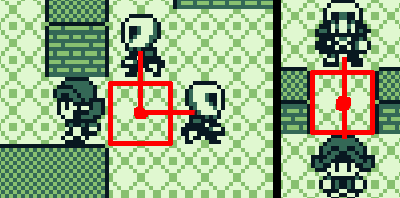
\includegraphics[width=0.5\textwidth]{include/images/desarrollo/special_cases.png}
\caption{Casos Especiales en Colisiones}
\label{figure:specialcases}
\end{figure}

En la captura de la \textbf{izquierda} lo que sucede es que \textbf{los dos enemigos calculan que deben ir a la misma casilla}, lo que provoca que terminen juntándose en ella. En la imagen de la \textbf{derecha}, el problema emerge cuando \textbf{el jugador quiere ir hacia arriba, pero el enemigo ya ha calculado que debe ir hacia abajo}.
\\ \\
El segundo caso lo vamos a conseguir corregir a tiempo para esta iteración. Lo que hacemos es lo siguiente: en el sistema de físicas, una vez recibimos un input, actualizamos al jugador y luego iteramos sobre todos las entidades. Esto nos deja una pequeña vía de escape en la cual podemos detectar que el jugador se está moviendo a la misma casilla que el enemigo tiene calculada, y poder impedir así que este último se mueva.

\begin{lstlisting}[caption={Comprobar Tiles y Denegar Movimiento}, label={code:checktiles}]
	ld 	 a, [_NPIXM]
	dec  a
	jr	 nz, .ps_move_en_up 		   ; Comprobamos que estamos en la primera iteración.

	call AI_CHECK_TILES 					; Comprueba que el jugador no está en la misma casilla

	ld 	 b, h
	ld 	 c, l

	or 	 a 									; Si no es 0, impedimos el movimiento.
	jp 	 nz, ps_en_mov_deny
\end{lstlisting}

Lo que se muestra en el código no es ni más ni menos que el \textbf{método de movimiento del enemigo}. Al comprobar en qué dirección se mueve el judador/a (y si es el primer frame del enemigo) se procede a comprobar si los tiles que tiene el jugador (los cuales ya están actualizados al haber realizado una iteración) son los mismos que a los que se tiene que mover.
\\ \\
El método de comprobación de tiles es muy simple: cogemos los tiles del jugador, los guardamos en el manejador de colisiones, y con la dirección del vector de enemigos apropiada comprobamos cada coordenada de los tiles. Si ambos son iguales, devolvemos un 1 para hacer saber al sistema de físicas que debe finalizar la ejecución.

\clearpage

\subsection{Mapas y Estados de Juego}

Como se diseñó en el GDD, el juego iba a constar de dos estados principales: el \textbf{mundo exterior y las mazmorras}. Con esta idea en mente, se van a incorporar al juego 3 mapas principales:

\begin{figure}[h]
\centering
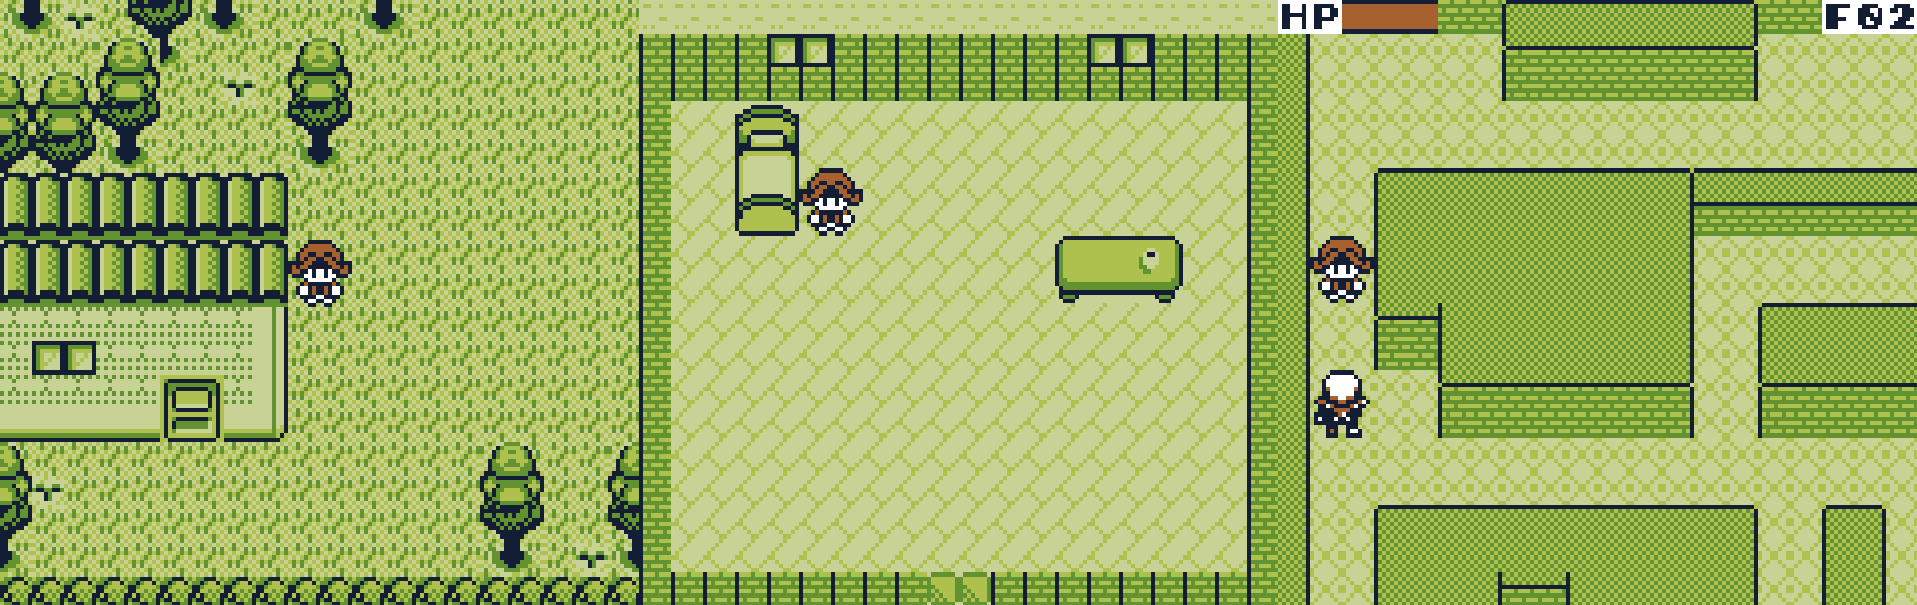
\includegraphics[width=1\textwidth]{include/images/desarrollo/states.png}
\caption{Mapas Principales}
\label{figure:states}
\end{figure}

\textbf{Dependiendo de en qué mapa} se encuentre el jugador, \textbf{activaremos unas mecánicas u otras}. Por ejemplo, en el mundo exterior el usuario no va a poder atacar, perder vida, pasar hambre, etc.
\\ \\
La implementación que se ha seguido para conseguir esto es la siguiente: una vez se detecta una casilla de tipo puerta, se pasa a comprobar su número de tile y se carga el mapa correspondiente. Como es probable que la pila siga teniendo returns pendientes que pueden afectar al gameplay, lo que hacemos es esperar una iteración entera, consiguiendo vaciarla. Para ello dispondremos de \textbf{dos bytes en RAM que indican si hay que cambiar de un estado a otro y a cuál}.

\begin{lstlisting}[caption={Mapas de Juego}, label={code:gamemaps}]
_STATE: 		DS 1 								; 0 = Overworld, 1 = Dungeon, 2 = Transition
_CHANGE: 		DS 1 							; bool to know if we have to change state

[...]

GM_SET_GAME_STATE:
	ld 	 [_STATE], a 									; Cambiamos el estado.
	ld 	 a, 1
	ld 	 [_CHANGE], a 								; Indicamos que tenemos que cambiar de estado.
	ret
\end{lstlisting}

\clearpage

Lo que hacemos a continuación, nada más entrar al bucle de juego, es \textbf{comprobar si debemos cambiar a ese estado} previo al comienzo de actualizar la inteligencia artificial, las físicas, animaciones, etc.

\begin{lstlisting}[caption={Bucle de Juego}, label={code:gameloop}]
[...]
.gameloop:		

	call GM_CHECK_STATE 						; Compruebo estado.
	call GM_UPDATE_INPUT 					; Actualizo inputs
	call RS_UPDATE 								; Actualizo renderizado
	call AS_UPDATE 								; Actualizo animaciones
	call AI_UPDATE 								; Actualizo inteligencia artificial

	call RS_WAIT_VBLANK 						; Espero al intervalo V-Blank
	call RS_DRAW 									; Dibujo sprites en OAM mediante DMA.
	call PS_UPDATE 								; Actualizo físicas.
	jp   .gameloop
\end{lstlisting}

\subsection{Conclusión}

En este caso creo que \textbf{el trabajo resultante no ha sido el esperado}. Me he encontrado con distintos problemas a lo largo de este período de tiempo que han perjudicado al desarrollo del proyecto. Esto quiere decir que, probablemente, voy a tener que \textbf{descartar alguna que otra tarea de la lista} para asegurarme de que lo más importante queda bien plasmado.

\clearpage

\section{Iteración 4 - Implementación de Elementos de Producto}

En esta iteración el \textbf{objetivo principal} ha sido el de \textbf{conseguir un producto}. Con esto veremos que el enfoque principal es el de hacer posible la muerte del jugador y el reinicio de partida, el paso de nivel, el poder matar enemigos, usar objetos, etc.

\subsection{Colisiones}

Nuevamente volvemos a hacer una \textbf{revisión de este aspecto} del juego. Ya no solamente para terminar lo que nos quedó por arreglar, si no para \textbf{rehacer el código de 0}.
\\ \\
Tras una mejor \textbf{analización del problema}, se llegó a la conclusión de que \textbf{tratar esta serie de problemas como casos especiales generaba demasiados "parches" en el código}. A parte, \textbf{ya existían métodos mucho más funcionales} que solucionaban todos los problemas de una vez.
\\ \\
La clave está en \textbf{guardarse en un array todas las casillas en las que los enemigos van a moverse o se han movido}. De esta forma, las entidades "reservan" casillas. Puede que parezca lo más lógico pero realmente es complicado caer en la cuenta de poder hacerlo de esta manera. \textbf{Juegos como \textbf{Pokemon: Mundo Misterioso} usan este método}.
\\ \\
Lo primero que debemos hacer es, como ya hemos dicho, crearnos un array donde vayamos a guardar todas las casillas reservadas. Es muy simple, \textbf{reservamos un espacio de 2 * Número de Entidades}.

\begin{lstlisting}[caption={Definición de Espacio para la Reserva de Casillas}, label={code:savetiles}]
_RESERVED_CELLS: DS MAX_ENTITIES*TILE_COORDS		; 2 Tiles * Maximum Number of Entities
\end{lstlisting}

Ahora, de manera \textbf{previa a que un enemigo calcule una casilla a la que ir}, va a \textbf{hacer la comprobación correspondiente para conocer si ya está reservada}. En caso de estarlo, pasaría a comprobar si puede moverse a otra.
\\ \\
A la hora de iterar sobre el array de casillas reservadas, no es conveniente malgastar memoria RAM poniendo a cada entidad un puntero a la posición de su casilla correspondiente.  Conforme vayamos iterando por entidad, con el índice del bucle sabremos qué posición exacta del vector corresponde a cada uno.
\\ \\
Una vez sabe la entidad a qué casilla debe moverse, la reservará para que, una vez llegados a la actualización de las físicas, comience a moverse \textbf{sin que haya otra entidad que pueda hacerlo también a esa misma posición}.

\begin{lstlisting}[caption={Reserva de Casillas}, label={code:reservetiles}]
AI_RESERVE_CELL:

	ld 	 hl, _RESERVED_CELLS 		; Posición inicial del vector de casillas reservadas.
	ld 	  a, [_TOTAL_EN] 					; Índice de la entidad actual.
	ld 	 de, 2 										; Número de coordenadas por casilla.
 	
ai_reserve_cell_loop:

 	dec  a
 	jr 	 z, ai_reserve_cell_do 			 	; Si nuestro índice es 1, vamos directamente a coger coordenadas.

 	add  hl, de 									; En caso contrario, sumamos el tamaño de casilla a la dirección de memoria.
 	jr 	 ai_reserve_cell_loop

ai_reserve_cell_do:
	; Get the saved tiles from the collision manager

	call CM_GET_TILEY 							; Cogemos coordenada Y
	ld 	 [hl], a 										; Guardamos coordenada Y
	inc  hl 											
	call CM_GET_TILEX 							; Cogemos coordenada X
	ld 	 [hl], a 										; Guardamos coordenada X
	ret
\end{lstlisting}

Como es lógico, en la iteración de la siguiente entidad lo que vamos a hacer es recorrer este mismo vector, de manera que comprobemos las coordenadas X e Y de la casilla a la que se intenta mover con todas las que ya hay reservadas. \textbf{En caso de que ambas coordenadas coincidan con alguna de ellas, impedimos el movimiento y probamos con otra}.

\subsection{Progresión de Juego}

Para conseguir un \textbf{producto} era de suma importancia tener algún tipo de \textbf{progresión dentro del juego}. En este tipo de juegos se consigue mediante el acceso a "pisos inferiores/superiores" del cual se encuentra actualmente el jugador (como podemos observar en la \textbf{figura \hyperref[figure:lifebar]{8.10}}). En este proyecto la propuesta inicial es la de conseguir \textbf{3 pisos en total}, más la última de todas donde se pueda pelear contra un enemigo final.
\\ \\
Para ello crearemos \textbf{una variable RAM en el manejador de partida}, que nos pueda indicar en qué piso nos encontramos actualmente. Dado este índice, \textbf{una vez detectemos que estamos en un tile especial} (el cual ya hemos nombrado en algún momento como escalera), \textbf{pasaremos a cargar el tilemap correspondiente}.
\\ \\
Para el cargado de tilemaps, al ser tan grandes, \textbf{debemos apagar y encender la pantalla LCD para evitar posibles corrupciones en el bus de vídeo}. El resultado que nos da es un efecto parpadeo no muy agradable a la vista, pero el cual \textbf{podemos solucionar con transiciones} (como veremos en el siguiente apartado).

\begin{figure}[h]
\centering
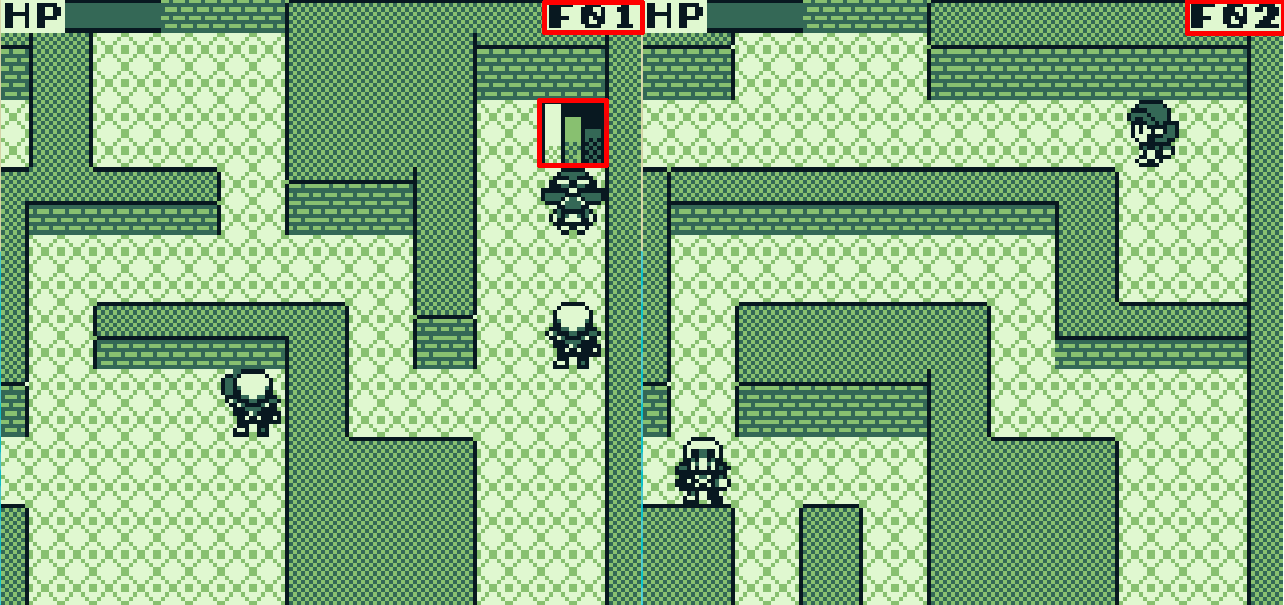
\includegraphics[width=0.8\textwidth]{include/images/desarrollo/level_progression.png}
\caption{Muestra Gráfica de Progresión de Juego}
\label{figure:levelprogression}
\end{figure}

Por último, todos los tilemaps (igual que con el que ya teníamos), los guardamos en ROM realizando su inclusión, y la cantidad de enemigos y objetos las creamos una vez comprobados en que nivel nos encontramos:

\begin{lstlisting}[caption={Carga de Niveles}, label={code:loadlevels}]
GM_INCREMENT_ACTUAL_FLOOR:
	
	ld 	 a, [_ACTUAL_FLOOR] 				; Cogemos indice de piso actual
	inc  a 														; Incrementamos el piso actual
	ld 	 [_ACTUAL_FLOOR], a 				; Guardamos el nuevo valor

	jp 	 RS_UPDATE_FLOOR_HUD 		; Actualizamos el HUD.

GM_GO_NEXT_FLOOR:

	call GM_INCREMENT_ACTUAL_FLOOR 		; Llamamos a la función de arriba
	
	; Eliminamos objetos y enemigos actuales.
	call EM_DELETE_ALL_ENEMIES
	call EM_DELETE_ALL_BLOCKS
	ld 	 a, [_ACTUAL_FLOOR] 							; Comprobamos que nivel tenemos que cargar
	cp 	 2
	jr 	 z, .floor2
	cp 	 3
	jr   z, .floor3
	ret
	[...]

.floor2: 																	; Cargamos piso 2
	ld 	 hl, Floor2 													; Dirección de inicio del tilemap
	ld 	 bc, Fin_Floor2-Floor2 							; Cantidad de bytes que ocupa el tilemap
	call RS_INIT_FLOOR 										; Dibujado del tilemap
	
	ld 	 hl, enemy_entity2 									; Creación de entidades
	call EM_CREATE_ENEMY
	[...]
\end{lstlisting}

\subsection{Transiciones entre Estados de Juego}

Como hemos comentado en el apartado anterior, el apagado y encendido de la pantalla LCD genera un efecto visual desagradable para el usuario. La mejor manera de solventarlo es mediante una \textbf{transición \textit{fade-in} y \textit{fade-out} de los colores}.
Este es un método que juegos como \textbf{Pokémon Rojo/Azul} ya utilizaban de manera constante para hacer pasar por desapercibidos los tiempos de carga de los distintos tilemaps.
\\ \\
La idea es sencilla: \textbf{por cada frame vamos a ir eliminando un color de nuestra paleta}. Esto quiere decir, por otro lado, que deberemos hacer distinción entre la Game Boy Original/Pocket y la Game Boy Color, puesto que la cantidad de colores (como ya hemos visto) es mucho más amplia en este último modelo.
\\ \\
Veamos el caso de las primeras Game Boy:
\\ \\
Como sabemos, la GB contiene un máximo de \textbf{cuatro colores}, los cuales van de más claro a más oscuro (teniendo en cuenta que los bits se cuentan de derecha a izquierda). Cada color se representa con 2 bits, siendo 11 el negro y 00 el blanco. Además, la paleta de sprites tiene la particularidad de que el color más claro, es en realidad transparente.

\begin{lstlisting}[caption={Paleta de Color en GB}, label={code:gbpal}]
BCK_PALETTE 	EQU %11100100 			; GB background palette
SPR_PALETTE 	EQU %11100000 			; GB sprite palette
\end{lstlisting}

Vamos a tener la necesidad de gestionar los primeros dos colores de la paleta de fondo de manera inversa. Esto se debe precisamente porque el primer color de la paleta de sprites es transparente, por lo que pongamos los bits que pongamos, el resultado va a ser el mismo. Al poner las dos paletas con los mismos colores, va a suceder lo siguiente:

\begin{figure}[h]
\centering
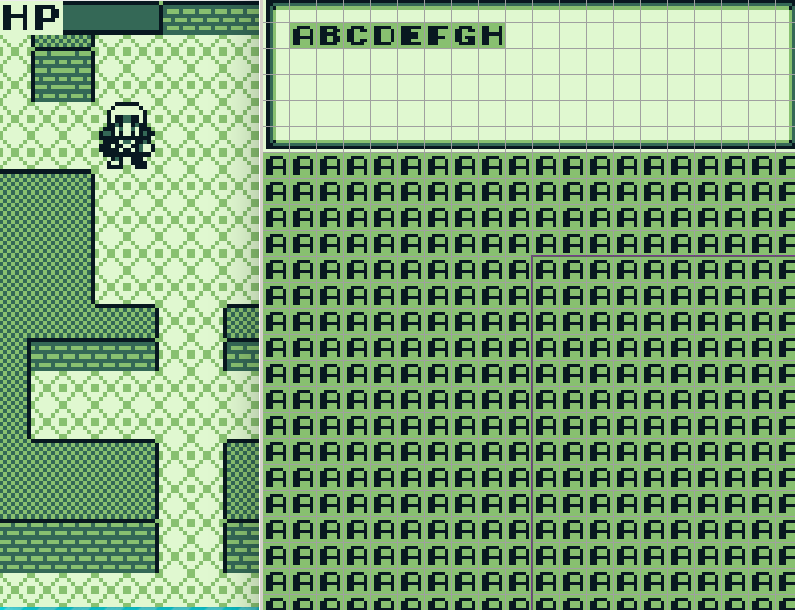
\includegraphics[width=0.5\textwidth]{include/images/desarrollo/pal_problem.png}
\caption{Problema con la Paleta de Color en GB}
\label{figure:transitiongb}
\end{figure}

Si nos fijamos bien, veremos que \textbf{los tiles de las letras, en el HUD tienen un fondo blanco, mientras que en el recuadro de la derecha tienen un fondo verde}. Esto se debe a que el color gris en la paleta de fondo es el color blanco en la de sprites.
\\ \\
Al final la solución es la de, \textbf{en el programa GBTD, intercambiar los colores de blanco a gris y viceversa en todos aquellos tiles que se utilizasen para el fondo} y el resto dejarlos igual. Ahora necesitaremos intercambiar estos dos mismos colores pero en el código. Todo esto provocaba que los tiles que utilizamos de sprites se viesen de la misma manera que si las utilizase de fondo, y que los demás tiles se viesen como tocaban.

\begin{lstlisting}[caption={Paleta de Color Invertida en GB}, label={code:gbpalinv}]
BCK_PALETTE 	EQU %11100001 			; GB background palette
SPR_PALETTE 	EQU %11100000 			; GB sprite palette
\end{lstlisting}

Volviendo al tema principal, lo que debemos hacer para conseguir la \textbf{transición a blanco} es, \textbf{por cada frame o iteración (en un total de 4 iteraciones), restar 1 a todos los colores}. De esta forma, el color negro pasa a gris, el gris a blanco, etc.
\\ \\
Por otro lado, en la \textbf{transición} de blanco \textbf{a color}, debemos ir \textbf{sumando 1 a todos los valores, mientras que los comparamos con el valor de la paleta original}. Una vez una componente sea igual que la de la paleta original, dejamos de incrementarla.
\\ \\
El \textbf{resultado} es el siguiente:

\begin{figure}[h]
\centering
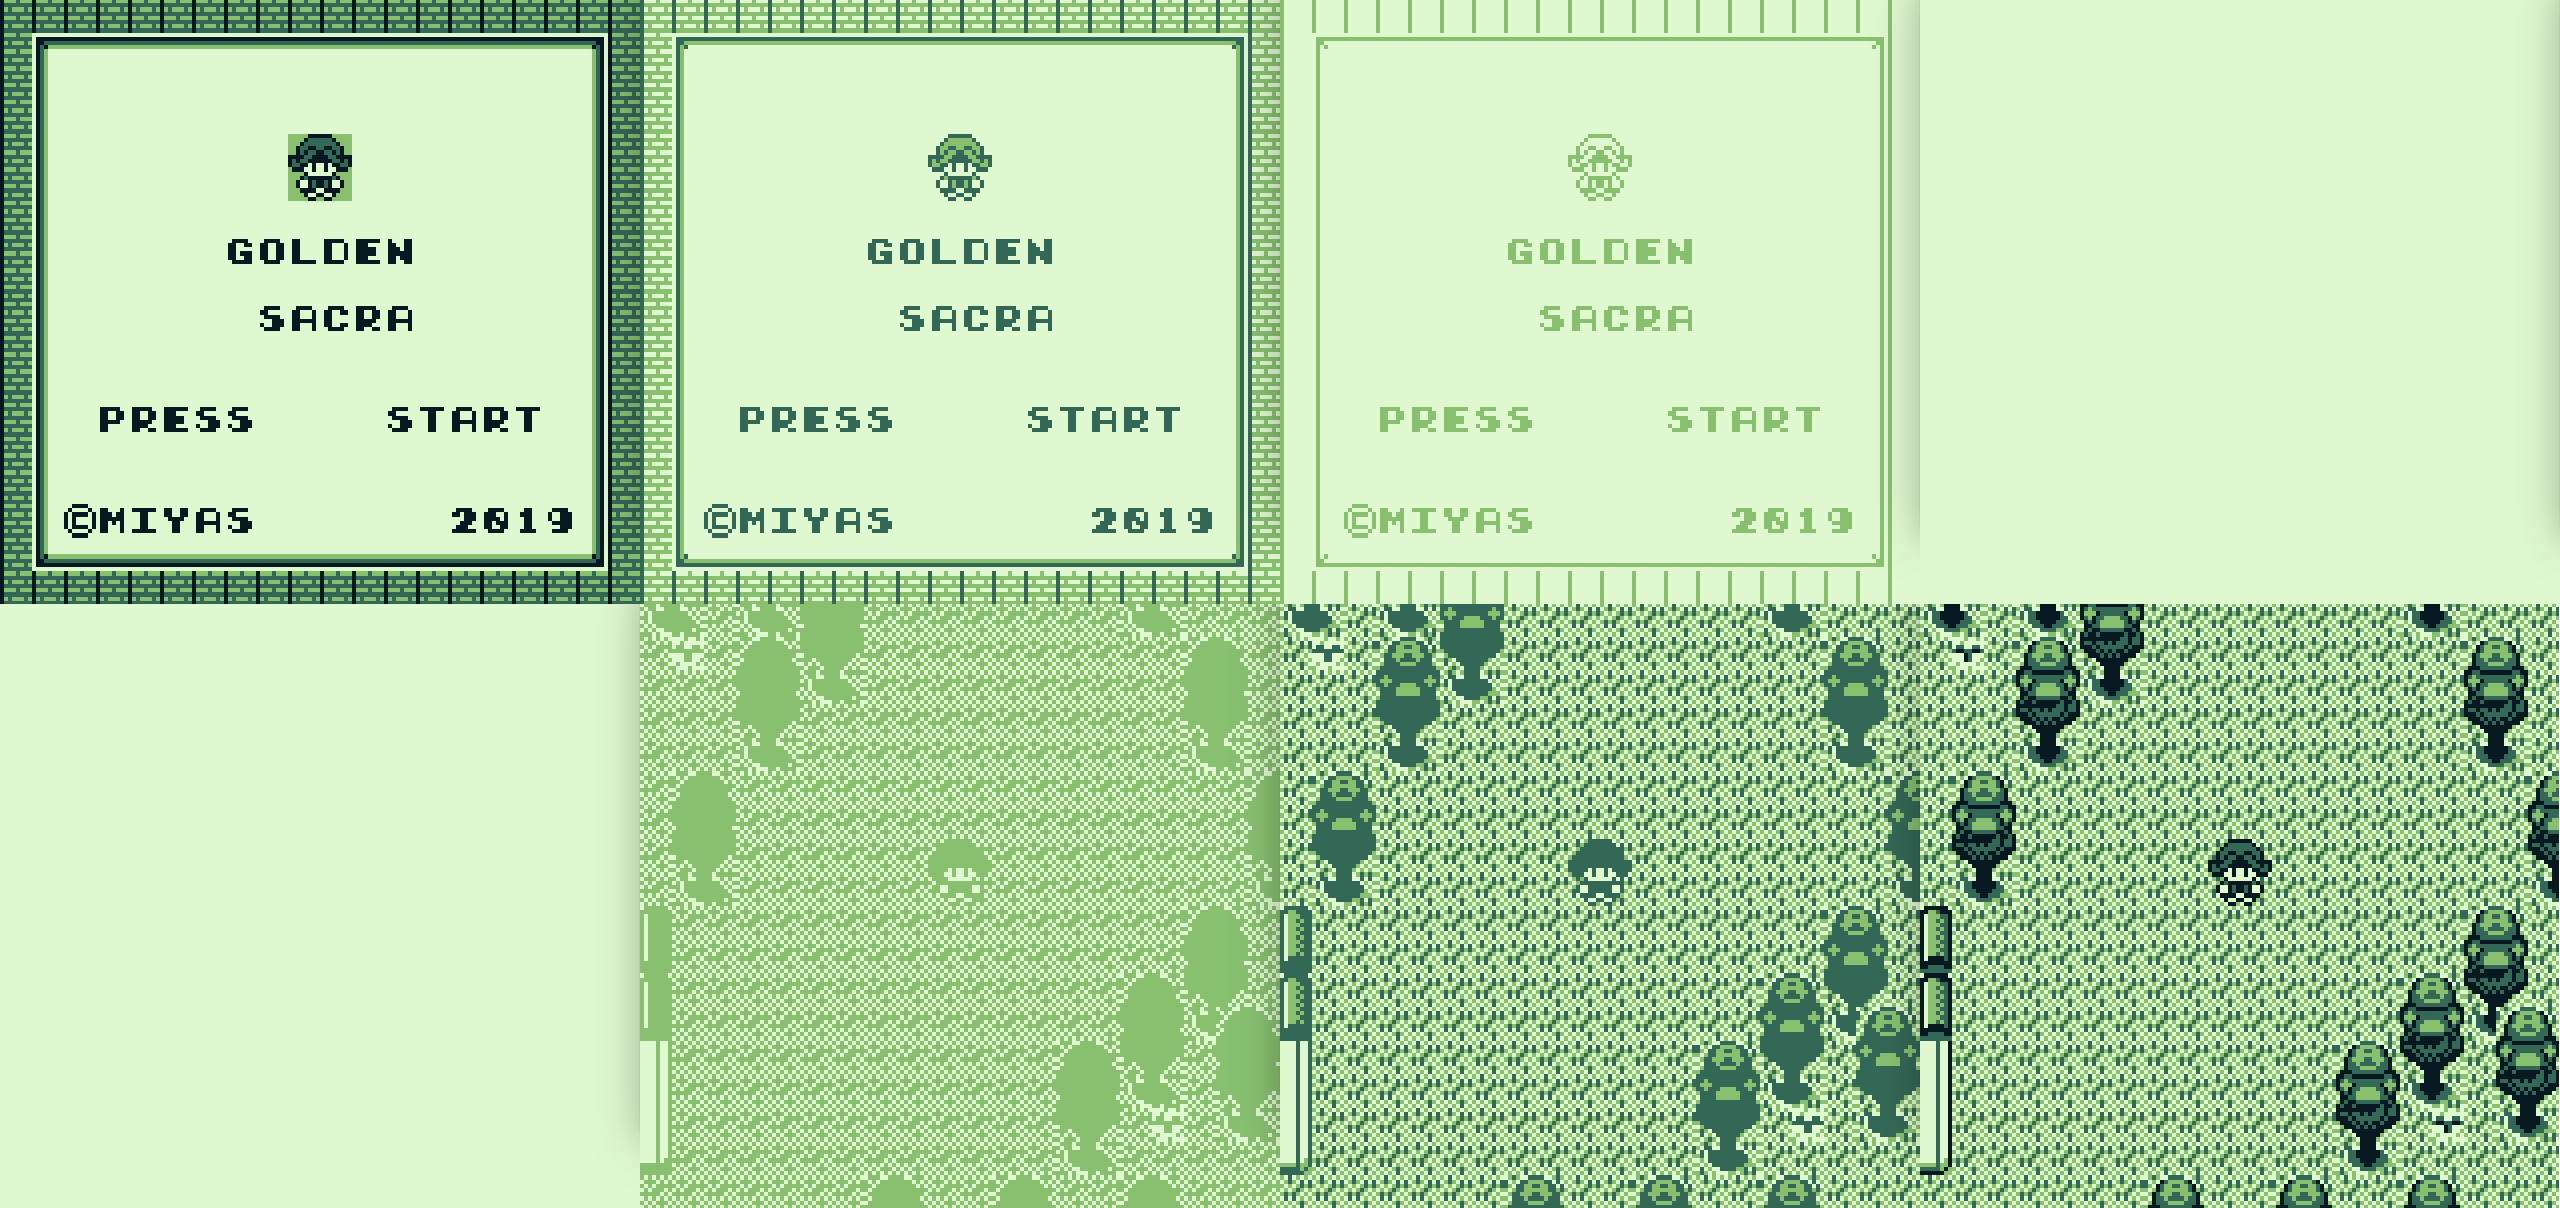
\includegraphics[width=1\textwidth]{include/images/desarrollo/fadeinout_gb.png}
\caption{Transición en Game Boy Original/Pocket}
\label{figure:transitiongb}
\end{figure}

Para el caso de la GBC la idea es exactamente la misma tanto para el \textit{fade-out} como para el \textit{fade-in}. La dificultad está en el comprender cómo gestiona los colores.

\begin{figure}[h]
\centering
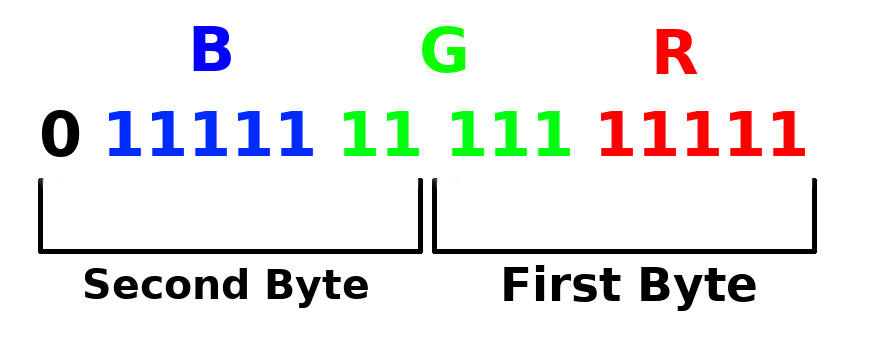
\includegraphics[width=0.6\textwidth]{include/images/desarrollo/gbcpalcolor.png}
\caption{Estructura de Color en GBC}
\label{figure:colorstructure}
\end{figure}

\textbf{El mayor problema es la componente G}, debido a que se halla intercalada entre el primer y el segundo byte. Como vemos además, cada componente dispone de 5 bits, lo cual nos da un total de \textbf{\(2^5\) posibilidades}, una vez más, \textbf{por componente}. Esto quiere decir que si, al igual que en GB, queremos conseguir el blanco absoluto en 4 iteraciones, \textbf{deberemos restar 1 a cada componente durante 32-1 iteraciones} (contamos el 0).
\\ \\
Para restar o sumar la componente G por separado, deberemos coger el primer byte, hacerle una operacion AND a los 3 últimos bits, efectuar 3 veces la operación RLC (o por el contrario, un SWAP y un RRC) para pasar los tres bits al principio del byte, y guardarnos el resultado. A continuación cogemos el segundo byte y nuevamente aplicamos un AND para guardarnos los dos primeros bits. Hacemos otro SWAP y otro RRC para no machacar los que tenemos en el segundo registro, y con una operación OR de ambos conseguimos la componente completa, la cual ya podemos decrementar. Para guardar de nuevo el valor tendríamos que efectuar justo los pasos marcados, pero a la inversa.

\begin{lstlisting}[caption={Conseguir Componente G de la Paleta de Color en GBC}, label={code:gcomponent}]
	ld   a, [hl] 							; a = GGGRRRRR
    and  %11100000	 						; a = GGG00000
    swap a 									; a = 0000GGG0
    rrc  a 									; a = 00000GGG
    ld   b, a 								; b = a
    inc  hl
    ld   a, [hl] 							; a = 0BBBBBGG
    and  %00000011 							; a = 000000GG
    swap a 									; a = 00GG0000
    rrc  a 									; a = 000GG000
    or   b 									; or = 000GGGGG
    ld   [_GBC_PAL_G], a 					; save green component in ram.
\end{lstlisting}

Como podéis apreciar, \textbf{esto es solamente para coger la componente verde} (a falta de todo lo demás), por lo que se genera mucho más código. Por ello es \textbf{importante comentar en cada operación el resultado esperado} y, de esta manera, evitar tener que ponernos a hacer trazas en caso de que algo vaya mal.

\subsection{Objetos y Hambre}

Este apartado estaba, al igual que los enemigos, hecho ya desde el primer prototipo a finales de la iteración 1. Esto conlleva, sin embargo, acarrear exactamente los mismos problemas.
\\ \\
La solución, por ende, es \textbf{crearnos nuevamente un array} (tanto en RAM como en DMA) de entidades que sean específicamente objetos. Y esto hay que cogerlo con pinzas porque es una decisión de diseño y estructuración del código.

\begin{lstlisting}[caption={Vector de Objetos}, label={code:itemarray}]
block_size  	= 7 	; AbsY, AbsX, Type, TileX, TileY, DMA Address [x2] (Little Endian).
block_dma_size 	= 4

dma_blocks:     DS 48   ; A 'block entity' could be an item, wich consists only of 1 sprite

num_blocks:     DS 1

last_dmabl_ptr: DS 2
last_block_ptr: DS 2

block_array: 	DS block_size*MAX_BLOCKS
\end{lstlisting}

Dentro del código este tipo de entidades las vamos a definir como "bloques" ya que \textbf{solo constan}, a diferencia del resto, \textbf{de un sprite} y pueden interactuar con el jugador (aquí la diferencia con los sprites de HUD).
\\ \\
La lógica de creación de la entidad, eliminación, etc. es la misma que la de los enemigos, por lo que no creo conveniente volver a explicarlo.
\\ \\
Por ahora, \textbf{conforme al Game Design Document}, vamos a disponer de \textbf{tres posibles objetos}, los cuales se encuentran esparcidos por el mapa. Esto nos obliga a agrandar el tamaño del jugador en \textbf{3 bytes más}, para saber con certeza cuántos disponemos de cada uno. Además, vamos a añadir un \textbf{cuarto byte como indicador de hambre} que tiene el jugador (mecánica descrita en el GDD).

\begin{lstlisting}[caption={Nuevo Tamaño del Jugador}, label={code:playernewsize}]
player_size 	= 10 	; Lifes, TileX, TileY, MovementDirection, LastMovement, Action, Hunger, Basic Potions, Super Potions, Basic Apples.
\end{lstlisting}

Como podemos observar, ahora disponemos de un byte respectivo para cada tipo de objeto.
\\ \\
Lo siguiente que debemos hacer es, \textbf{cada vez que el jugador termina un movimiento, comprobar si ha colisionado con alguno de los objetos que el array contiene}. Esto lo hacemos de una manera muy sencilla: comprobando las coordenadas X e Y de la casilla en la que se encuentran ambos. En el momento que demos con una coincidencia, comprobaremos el tipo de objeto y sumaremos 1 al byte correspondiente del jugador.

\begin{lstlisting}[caption={Actualizaciones a Final de Movimiento}, label={code:endmovement}]
PS_UPDATE_NPIXM:	
	[...]	
	call EM_INCREASE_PLAYER_LIFE 					; aumentamos la vida del jugador
	call EM_DECREASE_PLAYER_HUNGER 			; decrementamos el hambre

	call AM_RESET_PLAYER_SPRITES 					; reseteamos los sprites

	call EM_GRAB_ITEM 									; comprobamos si podemos coger un objeto.

	jp 	 AI_INIT
\end{lstlisting}

Una vez hemos obtenido el objeto, simplemente llamamos a la lógica de eliminación para que deje de ser visible en pantalla.
\\ \\
En el caso del hambre, por otro lado, lo que hacemos es decrementar el valor actual que tiene guardado el jugador y, de llegar a 0, comenzar a restar un valor mayor del que hemos sumado previamente al terminar el turno.

\begin{lstlisting}[caption={Actualización del Hambre}, label={code:updatehunger}]
EM_DECREASE_PLAYER_HUNGER:
	
	ld 	 e, pl_hunger
	call EM_GET_PLAYER_VARIABLE 				; Cogemos el hambre actual.
	or 	 a 														; Comprobamos que sea 0.
	jr 	 z, EM_DECREASE_PLAYER_LIFE 			; Si es 0, decrementamos la vida actual del jugador.

	dec  a 														; En caso de no ser 0, decrementamos el hambre.
	ld 	 [hl], a

	ret
\end{lstlisting}

A falta de los métodos de recuperar vida dado un input (para según qué objeto sumar un valor u otro) y el de recuperar hambre, este apartado se podría llegar a dar por finalizado. Para poder utilizar los objetos, \textbf{necesitamos un sistema de ventanas desde el cual dar la respectiva accesibilidad al jugador}.

\subsection{Ventanas - Diálogos y Menús}

La siguiente preocupación es el renderizado de ventanas. Como ya hemos comentado en la iteración 1, para poder dibujar una ventana debemos apagar y encender la pantalla LCD. Esto, al igual que ocurre con el cargado de niveles, \textbf{no se puede arreglar con una transición}.
\\ \\
Las primeras pruebas consistieron en esperar a un intervalo H-Blank o V-Blank y pintar de forma seguida 3 tiles en la segunda pantalla. Lo que sucedía era que al entrar \textbf{en V-Blank las pintaba sin problemas, pero en un intervalo H-Blank no le daba tiempo}.

\begin{figure}[h]
\centering
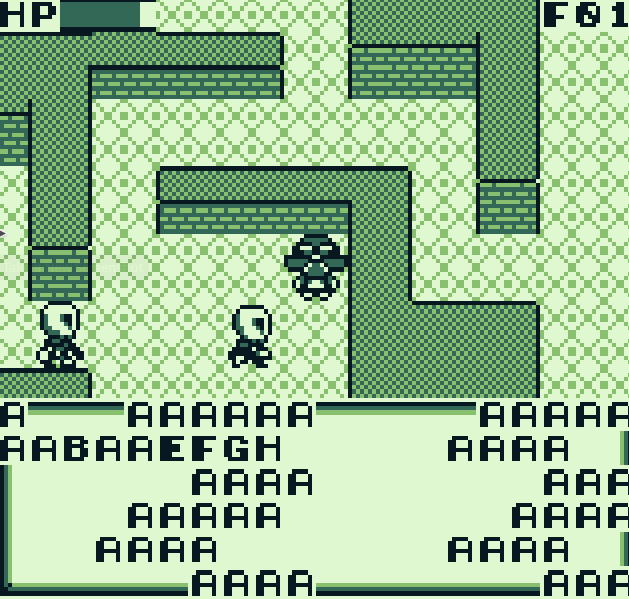
\includegraphics[width=0.5\textwidth]{include/images/desarrollo/windowproblems.png}
\caption{Problemas Dibujado de Ventanas Emergentes}
\label{figure:hudproblems}
\end{figure}

La \textbf{solución} fue \textbf{dejar a 1 la cantidad de tiles que se dibuja por intervalo H-Blank o V-Blank}, dando por asegurado que se iban a dibujar todas y cada una de las ventanas que se quisiesen.
\\ \\
Finalmente, la lógica del dibujado de ventanas funciona de la siguiente: nos pasan como \textbf{parámetros} un \textbf{ancho y un alto}. La esquina superior izquierda de la segunda pantalla siempre va a ser la esquina de una ventana, por lo que la iniciamos al tile que toca, y ponemos los tiles de borde superior un total de \(ancho-2\) veces (descontamos las dos esquinas). Ahora simplemente insertamos la esquina que falta. Hasta que no lleguemos a la última línea de todas, vamos a efectuar la misma operación: \(borde izquierdo - blanco*N - borde derecho\), (siendo \(N = ancho-2\). La última línea la hacemos idéntica a la primera, pero con los tiles inferiores. A continuación se muestra el código descrito:

\begin{lstlisting}[caption={Dibujado de Ventana}, label={code:drawwindow}]
RS_DRAW_WINDOW:

	ld 	 a, 33 						; Cargamos el ancho total + 1.
	sub  e 							; Le restamos el ancho pasado por parámetro.
	ld 	 [_OFFSET], a 			; Nos lo guardamos en RAM.
	
	ld 	 hl, _SCRN1 				; Cargamos la primera posición de la segunda pantalla.
	call RS_WAIT_MODE_01 					; Esperamos H-Blank o V-Blank.
	ld 	 [hl], CORNER_LU 							; Cargamos el tile de esquina superior izquierda.

	inc  hl 												; Incrementamos 1 vez la dirección de memoria.

	ld 	 d, e 												; Cargo en 'd' el Offset
	dec  d 												; Le resto 2
	dec  d

.rs_draw_window_loop_up:

	ld 	 c, 1 												; Cargo en 'bc' el número de bytes a copiar.
	ld 	 b, 0
	call RS_WAIT_MODE_01 					; Esperamos H-Blank o V-Blank
	ld 	 a, WINDOW_UP 							; Cargamos el tile de borde superior
	call RS_COPY_DATA 							; Input: a(var), hl(origin), bc(number of bytes)
															; Modified registers: hl, bc, af, e
	dec  d 												; Decremento 'd'
	jr 	 nz, .rs_draw_window_loop_up 	; Si 'd' no es 0, continuamos con el bucle.
	
	call RS_WAIT_MODE_01 					; Esperamos H-Blank o V-Blank
	ld 	 [hl], CORNER_RU 						; Insertamos la esquina superior derecha
	
	ld 	 a, [_OFFSET] 								; Recuperamos el Offset y lo insertamos en 'de'
	ld 	 e, a
	xor  a
	ld 	 d, a	 
	add  hl, de 										; Añadimos el Offset a la posición actual para llegar a la siguiente línea.
\end{lstlisting}

La \textbf{primera prueba}, como podréis comprobar en las capturas posteriores, fue \textbf{mostrar un pequeño texto en el momento que el usuario obtiene un objeto}, con el nombre de este. Para que todos los textos estuviesen organizados, hicimos un manejador nuevo que los guardase en ROM. Por lo general, lo que se suele hacer es guardar las cadenas de texto igual que en C++, pues el ensamblador lo pasa a bytes en tiempo de compilación. Después de eso, en tiempo de ejecución nos quedaría restarle al byte obtenido la primera posición de nuestro abecedario en memoria para coger el tile correspondiente. En este caso, \textbf{metimos directamente los bytes} correspondientes a los tiles que queríamos que saliesen.

\begin{lstlisting}[caption={Textos en ROM}, label={code:texts}]
; "Ashia got"
Item::
    DB 0, 18, 7, 8, 0, WHITE_TILE, 6, 14, 19
End_Item::

; "Basic Apple"
BasicApple:	
	DB 1, 0, 18, 8, 2, WHITE_TILE, 0, 15, 15, 11, 4
End_Basic_Apple:

[...]
\end{lstlisting}

Cada vez que el jugador escoja un objeto, sacaremos el texto "Ashia got" seguido del nombre específico. Vamos a hacerlo de la misma manera que hemos creado la ventana, con la única diferencia de que por cada tile que dibujemos, \textbf{aplicamos un delay de N frames} (al gusto del programador). En resumen: esperamos un número determinado de veces al intervalo V-Blank. Esta técnica la implementaban muchos juegos a la hora de mostrar diálogos.

\begin{lstlisting}[caption={Delay}, label={code:delay}]
RS_DELAY_FRAMES:
	ld 	 a, c 												; Cargamos en a el input (frames a esperar)
	or 	 a 												; Comprobamos que el parámetro sea distinto de 0.
	jr 	 nz, rs_delay_frames_vblank  		; Si no es 0, pasamos al bucle.

	jp 	 RS_WAIT_MODE_01 					; En caso de ser 0 esperamos a un H-Blank.

rs_delay_frames_vblank:

	call RS_WAIT_VBLANK 						; Esperamos al intervalo V-Blank.
	dec  c 												; Decrementamos el contador.
	jr 	 nz, rs_delay_frames_vblank 		; Si no es 0 volvemos al inicio del bucle.
	ret
\end{lstlisting}

El resultado es el siguiente:

\begin{figure}[h]
\centering
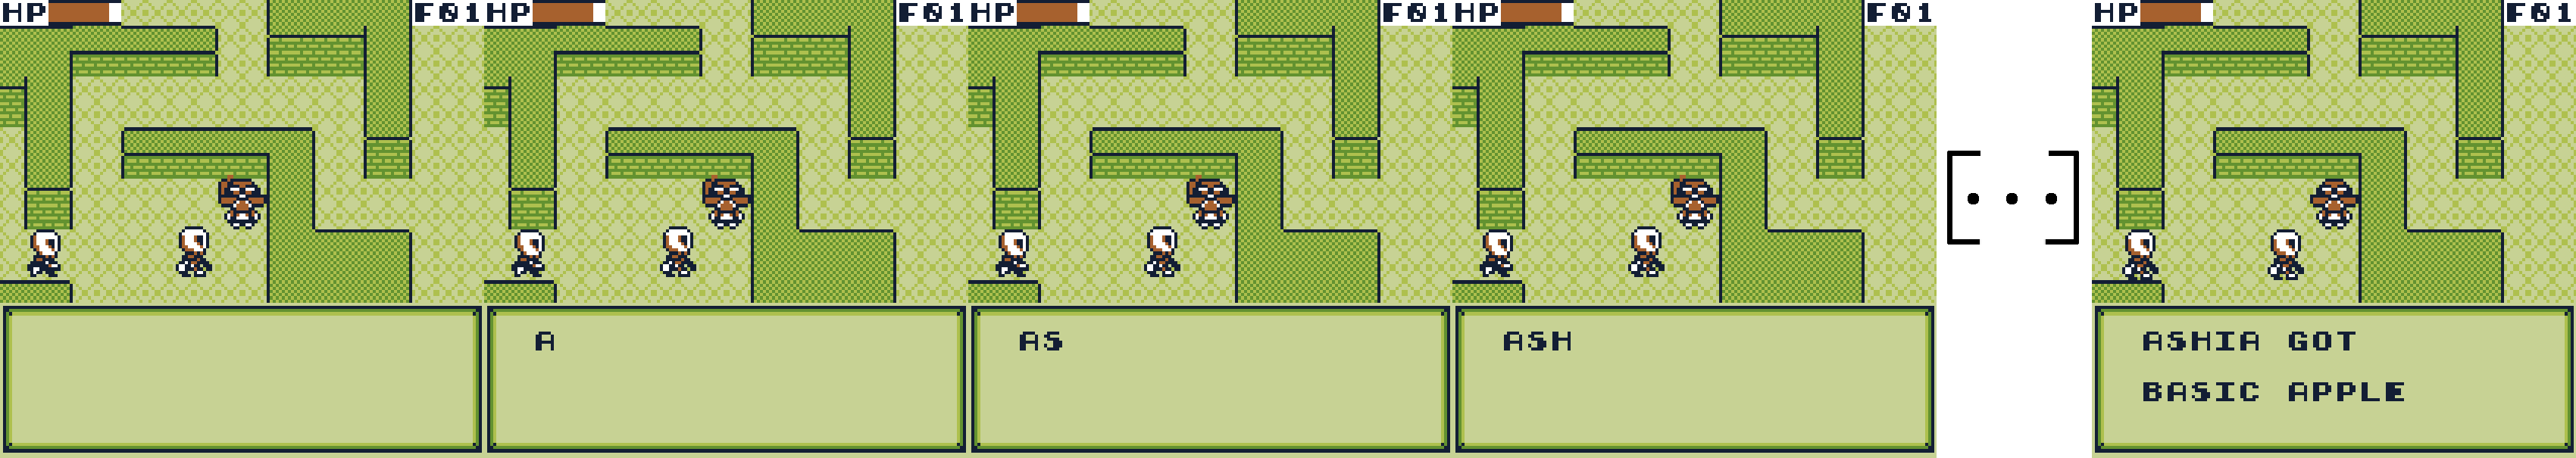
\includegraphics[width=1\textwidth]{include/images/desarrollo/dialogitem.png}
\caption{Dibujado de Textos}
\label{figure:drawtexts}
\end{figure}

Por último, algo que estaría bien comentar es la implementación realizada en este proyecto. Como ya hemos analizado previamente en el Estado del Arte, \textbf{la implementación de las entregas Pokémon Rojo/Azul se basan en el "copia y pega" de la pantalla secundaria a la primaria}. Por nuestra parte, \textbf{lo que hacemos es crear una única ventana que ocupe un ancho y un alto, con su esquina superior izquierda en la coordenada (0,0) de la segunda pantalla}. La ventaja es que el proceso es mucho \textbf{más rápido} a la hora de dibujarlo, pero tiene como inconveniente el de ser \textbf{incapaz de mostrar más de una ventana emergente} de forma simultánea.

\subsection{Conclusión}

Sin duda alguna siento que, hasta ahora, esta ha sido la iteración en la que \textbf{más trabajo se ha llevado a cabo}. Con esto prácticamente tengo el juego terminado a \textbf{falta de algunas mejoras} como pueden ser \textbf{efectos de sonido, retoques visuales, o alguna mejora en cuanto a inteligencia artificial}. Son, sin embargo, \textbf{tareas muy secundarias} que si se quedasen en el tintero no afectarían de manera grave al proyecto. Lo que sí necesito asegurarme ahora para que el producto sea totalmente jugable es que exista la posibilidad de utilizar los objetos esparcidos por el mapa.

\clearpage

\section{Iteración 5 - Diseño de Niveles para Enseñar al Usuario a Jugar}

En esta iteración el \textbf{objetivo principal} es terminar el \textbf{diseño de niveles} (objetos, obstáculos, enemigos...) de manera definitiva. Además, los primeros niveles del juego se deben pensar de forma que puedan guiar al jugador y enseñarle a jugar sin necesidad de más feedback.

\subsection{Actualización de RGBDS}

Como es lo normal en todo proyecto, con el paso del tiempo \textbf{las herramientas} que utilizamos \textbf{van obteniendo actualizaciones} que ofrecen al usuario todo tipo de mejoras y optimizaciones. De la misma forma, hay aspectos o nomenclaturas que tenemos en nuestro código y que los desarrolladores han creído conveniente dejar como obsoleto y reemplazarlos por otros.
\\ \\
Esto es precisamente lo que ha sucedido con este proyecto. Por suerte, los cambios no han afectado en gran medida.
\\ \\
Lo que se debe hacer en estas circunstancias es ir directamente a la \textbf{documentación oficial del desarrollador} y buscar los cambios que más nos interesen, como las eliminaciones:

\begin{figure}[h]
\centering
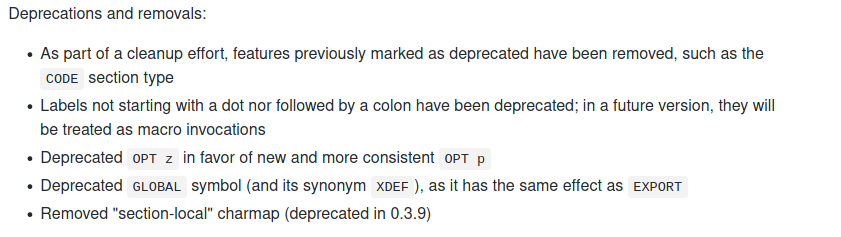
\includegraphics[width=1\textwidth]{include/images/desarrollo/rgbdsupdate.png}
\caption{Actualización 0.4.0 RGBDS - Código Obsoleto}
\label{figure:rgbdsupdate}
\end{figure}

Las \textbf{modificaciones importantes} fueron la \textbf{segunda y la cuarta}. La segunda lo que nos dice es que las etiquetas que empiecen con un punto se van a tratar como llamadas a una macro. Estos puntos los poníamos más por cuestiones estéticas que por otra cosa, ya que ayudaban a diferenciarlas como etiquetas interiores de una función.

\clearpage

La cuarta modificación cambió la forma de globalizar funciones y variables. \textbf{La nomenclatura "GLOBAL" dejó de existir} para dar paso a "EXPORT". A grosso modo no hay gran diferencia entre ellas y nuestro código debería funcionar perfectamente una vez hagamos el cambio.

\begin{lstlisting}[caption={Cambio de GLOBAL por EXPORT}, label={code:export}]
IF      !DEF(ENTITY_INC)
ENTITY_INC  SET  1

	;FUNCTIONS
	EXPORT EM_INIT
	EXPORT EM_CREATE_PLAYER
	EXPORT EM_CREATE_ENEMY

	[...]
\end{lstlisting}

\subsection{Utilización de Objetos}

Esta es una \textbf{tarea} que quedó \textbf{pendiente de la anterior iteración} y que era esencial para conseguir un producto jugable. La mayor complicación que podemos encontrarnos aquí es el dibujado de pantallas, ya que a parte de los iconos (utilizados para diferenciar los objetos entre sí), es el conseguir mostrar cuántas unidades de cada uno tiene el jugador en ese preciso instante. Por otro lado, \textbf{el dibujado de las ventanas quedó reducido al llamado de una función}, pasando por parámetro el ancho y el alto, así que en ese aspecto no deberíamos encontrar problema alguno.
\\ \\
Como ya se indicó en iteraciones previas, el jugador disponía de tres direcciones de memoria RAM, cada una para ir almacenando la cantidad que dispone de cada objeto. Cada vez que el jugador selecciona el objeto que desea utilizar, se comprueba esa variable dinámica, decrementándola en caso de ser distinta de 0. Justo después procedemos a aumentar la vida o el hambre del jugador, según qué caso.

\begin{lstlisting}[caption={Comprobación de Objeto Seleccionado}, label={code:selectedobj}]
	; THE PLAYER PRESSED A, so we check at which option he did.

	ld 	 a, [_OPTION]
	cp 	 1
	jp 	 z, rs_draw_inventory_check_apples 		; El jugador selecciona la manzana.
	cp   2
	jp 	 z, rs_draw_inventory_check_potions 	; El jugador selecciona la poción.
	cp 	 3
	jp 	 z, rs_draw_inventory_check_spotions 	; El jugador selecciona la súper poción.
	jp 	 RS_DRAW_MENU_BOX
\end{lstlisting}

\clearpage

¿Cómo mostramos el número exacto de unidades de cada objeto de las que disponemos? Si tenemos el número actual de un objeto en concreto, y tenemos el tile numérico inicial (el tile con el dibujo de un 0), \textbf{lo único que debemos hacer es sumar el número actual al número de tile para hallar el tile final que debemos mostrar}:

\begin{lstlisting}[caption={Muestreo}, label={code:selectedobj}]
	call EM_GET_PLAYER_VARIABLE 				; a = Número actual de manzanas
	ld 	 d, TILE_NUM_0 									; d = tile 0
	add  d												 	 	; Tile_0 + número de manzanas
	inc  bc
	ld 	 d, a
	call RS_WAIT_MODE_01 							; Modified registers:  a
	ld 	 a, d
	ld 	 [bc], a 													; Inserción del resultado en memoria de vídeo.
	ret
\end{lstlisting}

El resultado final se puede ver en la siguiente imagen:

\begin{figure}[h]
\centering
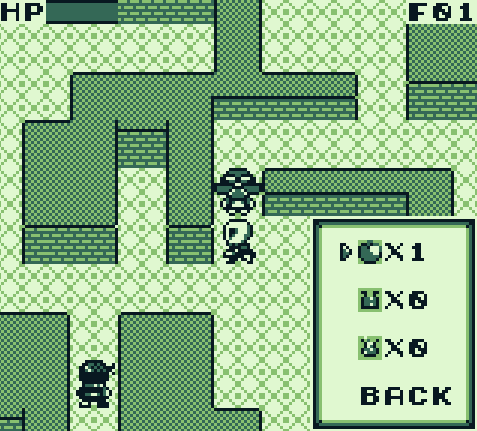
\includegraphics[width=0.5\textwidth]{include/images/desarrollo/Inventory.png}
\caption{Inventario}
\label{figure:inventory}
\end{figure}

\subsection{Múltiples Tilesets}

Ahora la idea es \textbf{introducir nuevos enemigos}. Esto implica añadir más tiles en nuestro tileset (bastantes más). Lamentablemente, \textbf{la GB es incapaz de tener en memoria tal cantidad} (recordemos que en nuestro tileset disponemos por el momento tanto de los carácteres alfabéticos, numéricos, sprites del personaje principal y sus animaciones, muros de la mazmorra, árboles, muebles, etc...). 
\\ \\
\textbf{Hay ocasiones en las que muchos de esos tiles no se utilizan para nada} y son memoria desperdiciada. Por ejemplo, dentro de la mazmorra no vamos a encontrar nunca tiles de árboles. Por este motivo, tenemos la obligación de diseñar 4 tilesets distintos y un cargado propio que, en función del estado de juego, cargue uno u otro.

\begin{lstlisting}[caption={Múltiples Tilesets}, label={code:multilesets}]
;==============================================================
; Tiles
;==============================================================
Persistent_Tiles:
	INCLUDE "./TILES/persistent_tiles.z80"
Persistent_Tiles_End:

Overworld_Tiles:
	INCLUDE "./TILES/overworld_tiles.z80"
Overworld_Tiles_End:

Dungeon_Tiles:
	INCLUDE "./TILES/dungeon_tiles.z80"
Dungeon_Tiles_End:

Title_Screen_Tiles:
	INCLUDE "./TILES/title_screen_tiles.z80"
Title_Screen_Tiles_End:
\end{lstlisting}

Además, aprovechando que dividimos el tileset principal en varios, podemos añadir más tiles que puedan ayudarnos a decordar los distintos paisajes del juego.
\\ \\
La forma en la que cargamos uno u otro es la siguiente: teniendo en cuenta que siempre tendremos en memoria los tiles del personaje, los números y las letras, nos creamos un \textbf{tileset llamado "persistent", que se va a mantener constante en todos los estados de juego}. Ahora, \textbf{sabiendo que} ese tileset \textbf{ocupa un total de N bytes}, podemos \textbf{cargar el siguiente a partir de la posición inicial de nuestra VRAM más ese tamaño N}:

\begin{lstlisting}[caption={Múltiples Tilesets}, label={code:multilesets}]
RS_GET_NONPERSISTENT_TILES_MA:
	ld	 hl, _VRAM 															; Memoria VRAM inicial
	ld	 de, Persistent_Tiles_End-Persistent_Tiles 			; Tamaño de N bytes
	add  hl, de 																; Dirección resultante en HL
	ret
\end{lstlisting}

Un problema con el que podemos llegar a encontrarnos es el siguiente: tenemos más tiles, y nos caben en la VRAM, ¿pero qué pasa si no nos cabe en la memoria ROM? Es decir, al fin y al cabo, todos esos bytes van a parar en la memoria de lectura, en algún momento nos quedaremos sin espacio, ¿no? Si esto sucede se nos mostrará en la terminal el siguiente mensaje:

\clearpage

\begin{figure}[h]
\centering
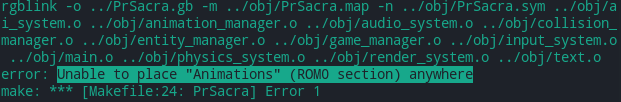
\includegraphics[width=1\textwidth]{include/images/desarrollo/NoRom.png}
\caption{Falta de Memoria ROM}
\label{figure:NoRom}
\end{figure}

\textbf{La solución es meterlo todo en ROMX}, ese banco de memoria que tenemos disponible y que hasta ahora no habíamos utilizado para nada. Poniendo las directrices de "SECTION", indicando el banco de memoria y poniendo a continuación los bytes a almacenar en ella, ya tendríamos el problema resuelto (al menos de momento).
\\ \\
El \textbf{segundo problema}: el \textbf{control de qué tileset está cargado y si hemos cargado los bytes que tocan}. Esto realmente no es un problema como tal, sino un descuido por parte de nosotros, los programadores. Hay que llevar cuidado en todo momento ya que se pueden producir efectos tan adversos como el que se muestra a continuación:

\begin{figure}[h]
\centering
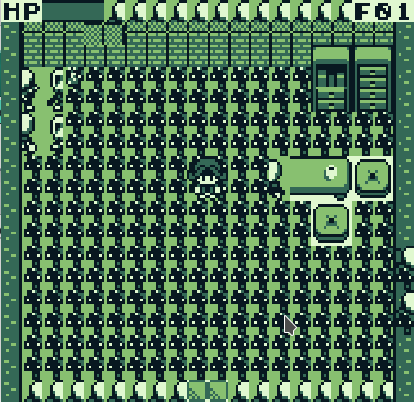
\includegraphics[width=0.5\textwidth]{include/images/desarrollo/wrongtileset.png}
\caption{Cargado Erróneo de Tileset}
\label{figure:wrongtileset}
\end{figure}

El \textbf{tercer y último problema}: si en nuestro tileset inicial tenemos unos números de tile específicos por los cuales permitimos dejar al jugador interaccionar de alguna forma,\textbf{ ¿qué ocurre si tenemos más de un tile con el mismo número?} Por ejemplo, supongamos que el tile de suelo es el 103 en nuestro tileset inicial. Ahora lo dividimos en varios y tenemos que nuestro tile de suelo es el 50. Perfecto, esto se debe a que tenemos menos tiles en general. Pero, lamentablemente, en el otro tileset también tenemos un tile con número 50, y a este último también nos vamos a poder mover. ¿Cómo lo solucionamos? Es cuestión de diseño más que de programación. En este caso colocaremos en ese número otros tiles a los que el jugador no pueda llegar nunca, o que (por el contrario) también sea un suelo.
\\ \\
Aprovechando que podemos insertar muchos más tiles, nos podemos permitir el lujo de gastar algo de tiempo en el diseño de la pantalla principal del juego, la cual ha quedado así:

\begin{figure}[h]
\centering
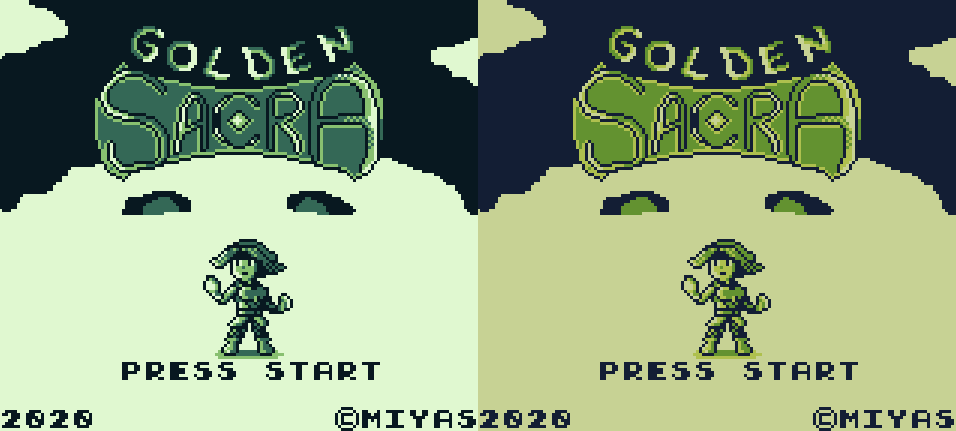
\includegraphics[width=0.7\textwidth]{include/images/desarrollo/title_screen.png}
\caption{Pantalla Principal de Juego Definitiva}
\label{figure:titlescreen}
\end{figure}

\subsection{Inserción de Objetos y Enemigos}

Este apartado es el que \textbf{más trabajo} ha tenido y el que \textbf{más corto va a ser de explicar}. Principalmente teníamos la idea de crear una inteligencia artificial, pero analizando el tiempo del que disponemos y el resto de entregas del mismo género, es preferible tirar de elementos básicos en cualquier RPG como pueden ser la cantidad de vida y el daño de un enemigo.
\\ \\
Con esto en mente,  hemos diseñado 3 enemigos más para poder hacer una \textbf{dificultad ascendente} según el jugador fuese progresando por los distintos niveles.

\begin{figure}[h]
\centering
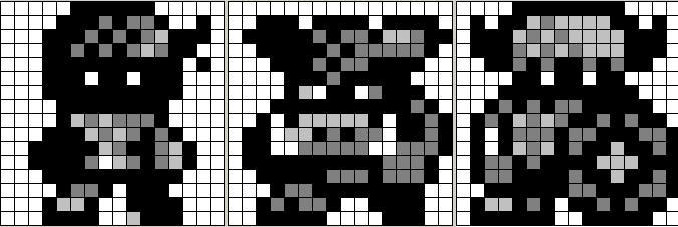
\includegraphics[width=0.7\textwidth]{include/images/desarrollo/newenemies.jpg}
\caption{Diseño de Nuevos Enemigos}
\label{figure:newenemies}
\end{figure}

De esta manera, \textbf{el primer enemigo tendría más vida pero menos daño que el enemigo inicial, el segundo tendrá la misma vida pero más daño, y el tercero tendrá más vida y más daño}. Así mismo, mostrando cada enemigo en un nivel nuevo,  podemos tener esa dificultad escalonada que buscamos. 
\\ \\
Lo único que nos queda es calcular en qué sitios meter qué objetos para no hacer imposible el avance en el juego, pero sí que te haga decidir si es rentable o no el hacerte con él. Y lo más importante de todo: procurar que el juego sea divertido.

\begin{figure}[h]
\centering
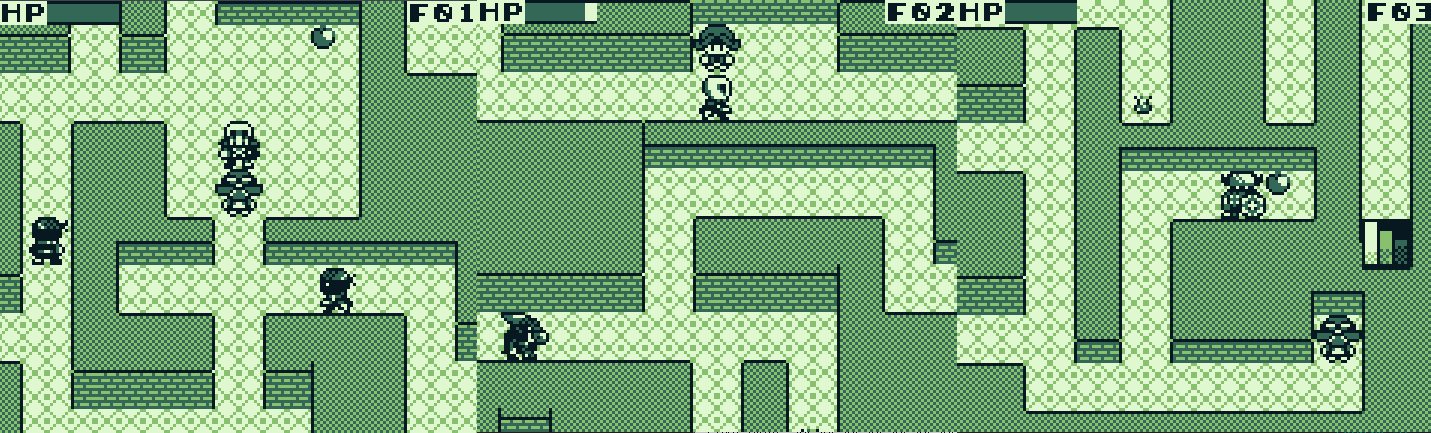
\includegraphics[width=1\textwidth]{include/images/desarrollo/leveldesign.png}
\caption{Diseño de Niveles}
\label{figure:leveldesign}
\end{figure}

¿Por qué se ha comido tanto tiempo esta tarea? Porque se necesita de mucho diseño y prueba y error para \textbf{comprobar que todo funciona como debe y que el juego no es frustrante ni imposible}. Además, para meter cada enemigo u objeto se necesita calcular de manera previa las coordenadas X e Y que van a tener, así como los tiles en los que se va a encontrar.

\subsection{Conclusión}

Pese a la situación en la que nos encontramos la mayoría de personas actualmente, me puedo dar con un canto en los dientes al haber conseguido sacar el trabajo adelante. La motivación ha sido un factor clave a la hora de seguir con el desarrollo del proyecto.
\\ \\
Me \textbf{quedan dos iteraciones más a lo sumo} y no tengo duda alguna de que el proyecto esta en buenas condiciones. Como dije en la conclusión de la iteración 4, \textbf{las tareas que faltan son secundarias, pero van a servir para dejar un producto completo y cerrado}, el cual se pueda meter a un cartucho físico y vender.

\clearpage

\section{Iteración 6 - Mejoras Gráficas, Gameplay y Efectos de Sonido}

Esta iteración (de unas dos semanas de duración) se ha dedicado a la mejora tanto de elementos gráficos pertenecientes al HUD, como de inteligencia artificial y música. Al ser la penúltima iteración antes de la entrega del proyecto, a parte de lo ya nombrado, otro objetivo ha sido el de arreglar distintos errores que hacía que el juego se congelase en distintas ocasiones.

\subsection{Música y Efectos de Sonido}

Ya habíamos visto en la iteración 1, podemos hacer sonar un "Do Re Mi Fa Sol La Si" constante a través del canal 1. Sin embargo, es un sistema que nos limita mucho a la hora de ser capaces de implementar música o distintos efectos de sonido según que evento se dé dentro del juego.
\\ \\
Vamos a utilizar ahora todos los canales de audio (a excepción del tercero), y además no vamos a utilizar parámetros fijos de frecuencias, longitud, ciclo de trabajo o envolventes. Cada nota tendrá sus 3 o 4 bytes (dependiendo del canal) que nos ayudarán a tener una mayor variedad de resultados.
\\ \\
Dicho esto, lo primero que he modificado ha sido la manera en la que se toca una nota. Como vamos a hacer uso de los canales 1, 2 y 4, he creado los tres métodos distintos en los que, dada una dirección de memoria, coge los 3 o 4 bytes contiguos para meterlos en sus registros correspondientes:

\begin{lstlisting}[caption={Método de Sonido en Canal 1}, label={code:channel1sound}]
AS_PLAY_NOTE_CHANNEL_1:

    ld   a, [hl]
    ld   [rNR10], a
    inc  hl
    ld   a, [hl]
    ld   [rNR11], a
    inc  hl
    ld   a, [hl]
    ld   [rNR12], a
    inc  hl
    ld   a, [hl]
    ld   [rNR13], a              
    inc  hl
    ld   a, [hl]
    ld   [rNR14], a

    ret
\end{lstlisting}

Con esto, para generar los efectos de sonido, solamente tendríamos que hacerle la llamada en cualquier otra parte del código con la dirección de memoria correspondiente en HL. Aquí el tempo o la nota actual a tocar son completamente innecesarias ya que queremos que se produzcan de forma inmediata.
\\ \\
Para hacer la banda sonora del juego, por otro lado, sí que vamos a necesitar de un sistema algo más complejo. Lo que tomábamos antes como "nota actual" era el número a sumar a una dirección de memoria específica. En esa dirección de memoria resultante, es donde realmente estaba la nota a tocar. ¿Qué ocurre si para llegar a la siguiente nota necesitamos sumar un número de más de 8 bits? ¿Y más de 16 bits? La escalabilidad es mínima, por lo que tendremos que cambiar lo que la "nota" simbolizaba a, simple y llanamente, una dirección de memoria fija. Vamos a seguir con el ejemplo del canal 1: 

\begin{lstlisting}[caption={Método de Música en Canal 1}, label={code:channel1music}]
AS_PLAY_MUSIC_CHANNEL_1:

    ld   a, [_NOTA]               	; Cargamos la dirección de memoria de la nota actual a tocar
    ld   l, a                    
    ld   a, [_NOTA+1]
    ld   h, a
    ld   a, [hl]                 

    cp   _KEEPNOTE 			; Comprobamos si debemos cambiar de nota, hacer un silencio o mantenerla.
    jr   z, as_note_end_keep

    call AS_PLAY_NOTE_CHANNEL_1

as_note_end_keep:

	; Mantenemos la nota.
    [...]
    
    ; Comprobamos si era la última nota. Reseteamos o continuamos a la siguiente
    [...]
	jr 	 z, as_note_end_reset
	
as_note_end_not_reset:

    ; Actualizamos la dirección de memoria de la nota a la siguiente.
    [...]
	
	ret
	
as_note_end_reset:

    ; Reseteamos la dirección de memoria de la nota a la primera.
    [...]

    ret
\end{lstlisting}

El único parámetro de entrada que le tenemos que pasar a la función es la dirección de memoria final de la canción que está sonando en BC. Al ser música de fondo que suena constantemente en el juego, el único momento en el que nos vamos a preocupar de cambiar la nota inicial de la canción es en los cambios de estado de juego (pantalla de título, mazmorra, etc...).
\\ \\
Al igual que hacíamos con los gráficos, las canciones y efectos de sonido también los vamos a guardar en el banco de memoria secundario ROMX:

\begin{lstlisting}[caption={Música y SFX en ROMX}, label={code:musicromx}]
TITLE_SCREEN1:
    DB $00, $00, $00, _SILENCE, _SILENCE
    DB $00, $00, $00, _SILENCE, _SILENCE
    DB $00, $81, $4B, _A, _OCT6_NR
    DB _KEEPNOTE
    DB $00, $8A, $47, _G, _OCT6_NR
    DB $00, $00, $00, _SILENCE, _SILENCE
    DB $00, $81, $4B, _C, _OCT7_NR 
    DB _KEEPNOTE
    DB _KEEPNOTE
    [...]
END_TITLE_SCREEN1:

[...]

OBJECT_SOUND::
    DB $00, $C0, $43, $44, $87
TEXT_OBJECT_SOUND::

[...]

; CHANNEL 4

DAMAGE_SOUND::
    DB $00, $F1, $61, $C0
END_DAMAGE_SOUND::
\end{lstlisting}

¿Y cómo sabemos qué combinación de bytes colocar para que suene un sonido en concreto? Aquí es donde entra la herramienta de GBSound Sample Generator, como bien muestro en la sección de \hyperref[GBSound]{\textbf{herramientas utilizadas}}.
\\ \\
Como podemos observar, en los bytes de \hyperref[code:musicromx]{\textbf{\_TITLE\_SCREEN1}} disponemos de distintas nomenclaturas como \textit{\_SILENCE} o  \textit{\_OCT6\_NR}. Simplemente se tratan de distintas frecuencias que nos dan las octavas y notas que queremos. Por ejemplo, un \textit{\_A} seguido de un \textit{\_OCT6\_NR} nos daría la nota La en Octava 6. Las últimas dos letras se utilizan para activar o desactivar el bit que impide que la nota se mantenga constante a lo largo del tiempo, sin llegar a efectuar su estado de relajación.
\\ \\
Una pregunta que nos podemos llegar a hacer es la siguiente: ¿Por qué no analizar el código de juegos como Pokémon Rojo para saber cómo tienen programado el sistema de audio? Aquí entramos en temas de tiempo y necesidad. En este proyecto el realizar un sistema de audio completamente funcional es algo que se quedaba en un plano muy secundario. Como partíamos de una base (lo realizado en la iteración 1) solo se ha necesitado comprobar cuáles eran las necesidades y efectuar las respectivas modificaciones. Obviamente, esto no quiere decir que el analizado de distintas entregas sea una pérdida de tiempo. Seguramente haciendo esto último podamos llegar a tener un sistema mucho más complejo, el cual nos permita disponer de más funcionalidades. Aún así lo reitero: no es el principal objetivo de este proyecto.
\\ \\
Todo lo que necesitamos ahora es imaginación y gusto musical con el que componer una canción y transcribirla a bytes. En el caso de que nos falte alguna de las dos cualidades, siempre podemos recurrir a páginas web como Fiverr en la que podremos encontrar distintos artistas que nos van a hacer un buen trabajo. Marc Davis fue, en este caso, el artista que compuso las canciones de este proyecto. Todo lo que él necesitaba era alguna captura del proyecto y referentes sobre los que inspirarse.

\begin{figure}[h]
\centering
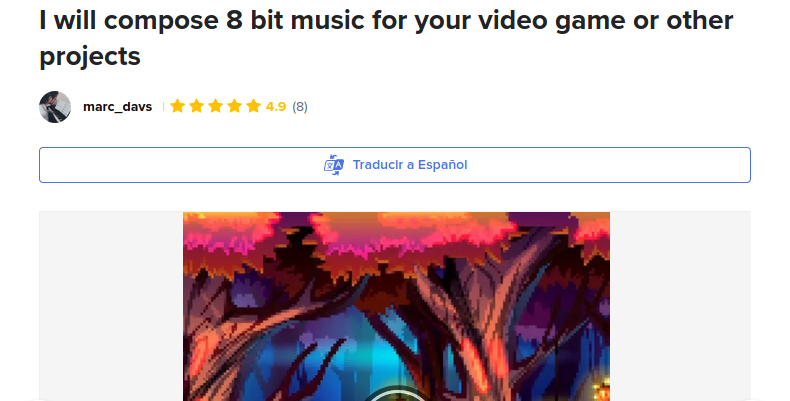
\includegraphics[width=0.7\textwidth]{include/images/desarrollo/marcdavs.png}
\caption{Marc Davis - Compositor Musical en Fiverr}
\label{figure:marcdavs}
\end{figure}

Este es un trabajo de ingeniería y, por tanto, no es nuestro trabajo el realizar la composición de una banda sonora. Es por ello que, en casos como estos, podemos hacer uso de fuentes externas (siempre y cuando tengamos en cuenta los derechos de uso).

\subsection{Arreglo Visual en Ventanas Emergentes}

Las ventanas emergentes que se realizaron en la iteración anterior no quedaron del todo usables debido a un problema visual en el que los sprites, al estar siempre por encima de las dos pantallas de fondo, ocultaban parte de los textos:

\begin{figure}[h]
\centering
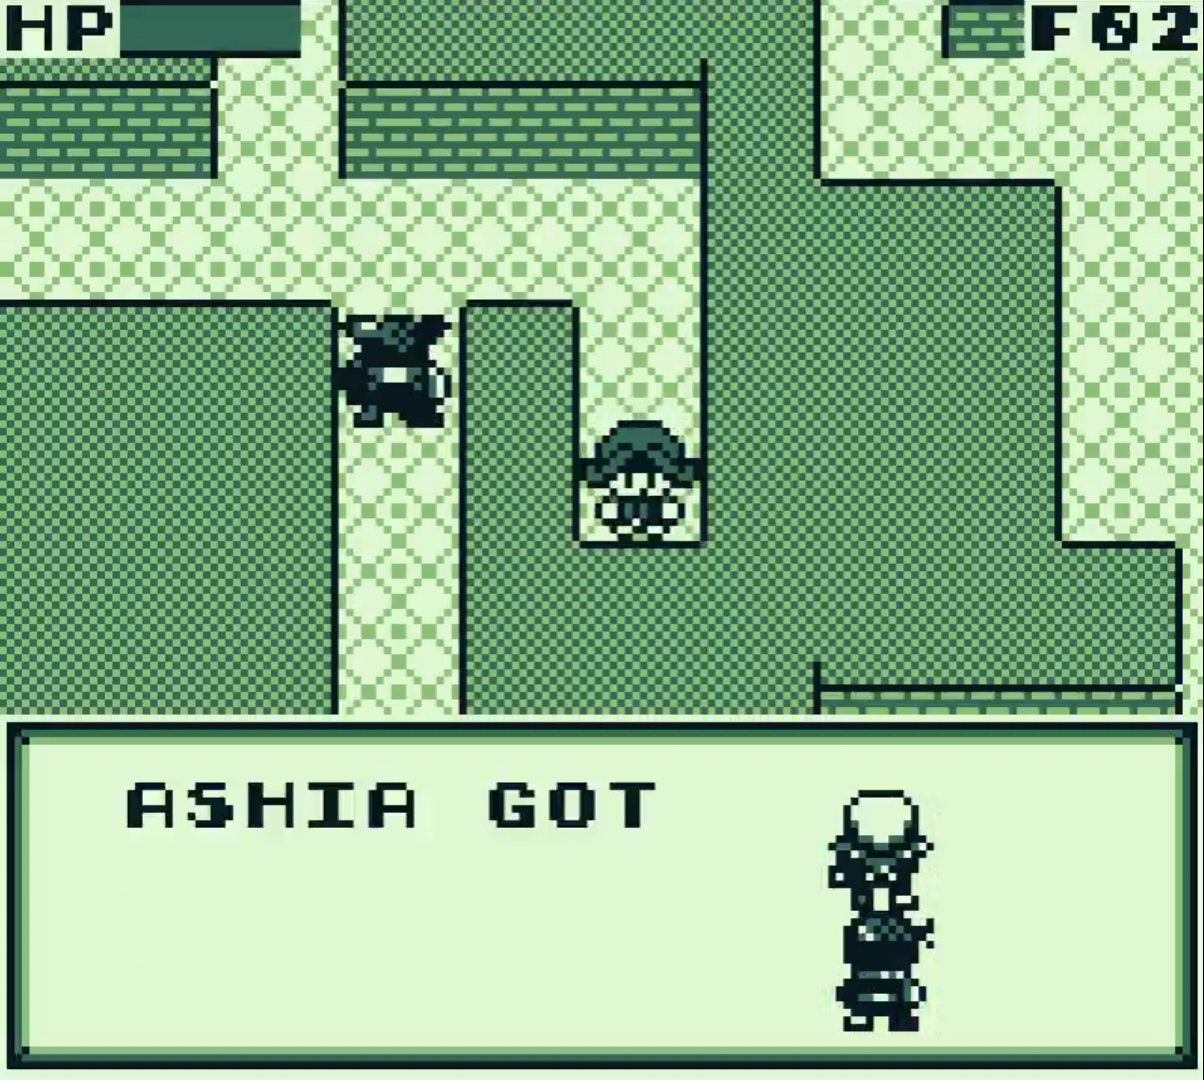
\includegraphics[width=0.5\textwidth]{include/images/desarrollo/hudissue.png}
\caption{Problema Visual Ventanas Emergentes}
\label{figure:hudissue}
\end{figure}

Para solucionar este problema, lo que debemos hacer es comprobar las coordenadas en tiles de cada sprite, tanto del jugador, como enemigos y objetos. Por ejemplo, en la imagen \hyperref[figure:hudissue]{\textbf{8.28}} tendríamos que comprobar que la coordenada Y fuese menor de N, mientras que (en este caso) la coordenada X nos es indiferente.
\\ \\
Con esto en mente, ya sabemos que la función que hagamos va a necesitar dos parámetros: las coordenadas X e Y mínimas por las cuales, si un sprite está por encima de ellas, lo tendremos que esconder.

\begin{lstlisting}[caption={Escondido de Sprites Según su Tile}, label={code:hidesprite}]
RS_HIDE_SPRITES:

	xor  a
	call PS_SET_UPDATE_ABSOLUTES 	; Impedimos que se actualicen en el render.

	call EM_GET_ENEMIES_ARRAY 				
	call rs_hide_sprites_start 				; Escondemos los enemigos

	call EM_GET_BLOCKS_ARRAY
	call rs_hide_sprites_start 				; Escondemos los objetos

	jp 	 RS_DRAW 									; Una vez terminado, redibujamos todo.

rs_hide_sprites_start:

	or 	 a 												; Comprobamos si hay al menos 1 entidad.
	ret  z

	[...]

rs_hide_sprites_loop:

	ld 	 a, [hl] 									; HL = Y component
	sub  c 	 									; E_Y - Minimum_Y
	jr 	 c, rs_hide_sprites_next 	 	; Si el resultado no da acarreo, significa que la entidad no está por encima del mínimo Y.

	inc  hl 										; HL = X component
	ld 	 a, [hl] 									
	sub  b 										; E_X - Minimum_X
	jr 	 c, rs_hide_sprites_next 		; Si el resultado no da acarreo, significa que la entidad no está por encima del mínimo X.

	; Si las coordenadas son mayores a los mínimos, lo escondemos. Para ello ponemos a 0 sus coordenadas en el DMA.

	xor  a
	ld   [hl], a 								; X = 0
	dec  hl
	ld 	 [hl], a 								; Y = 0
	
rs_hide_sprites_next:

	; Sumamos a la dirección HL actual un número específico que nos de el primer valor de la siguiente entidad.
	[...]

rs_hide_sprites_next_entity:
	
	; Comprobamos si nos quedan más entidades. En caso afirmativo, actualizamos la dirección HL.
	[...]
	
\end{lstlisting}

En el código expuesto no se muestra cómo se esconde al jugador. Esto se debe a que, mientras que a los enemigos y objetos se les actualizan las coordenadas de pantalla (o coordenadas absolutas) por ciclo de ejecución, al jugador no. Quiere decir que, a las dos primeros, con poner en el DMA los valores de las coordenadas a 0 van a dejar de aparecer en pantalla y una vez terminado todo, el juego va a coger las coordenadas guardadas en cada entidad y las va a volver a poner en la OAM. Si hiciésemos esto con el jugador veríamos que los sprites se esconden, pero no se vuelven a poner en su sitio. Para poder esconderlo tendremos que manipular la OAM de forma directa:

\begin{lstlisting}[caption={Escondido de Sprites Según su Tile}, label={code:hidesprite}]
RS_HIDE_PLAYER_SPRITE:
	
	ld 	 de, _OAMRAM 			; Dirección inicial de la OAM
	ld   a, 4
	ld 	 [_COUNT2], a
	ld 	 a, 1 								; Número de entidades a comprobar

	jr 	 rs_hide_sprites_start ; Llamada al método anterior.
\end{lstlisting}

El resultado lo podemos ver en el siguiente par de imágenes:

\begin{figure}[h]
\centering
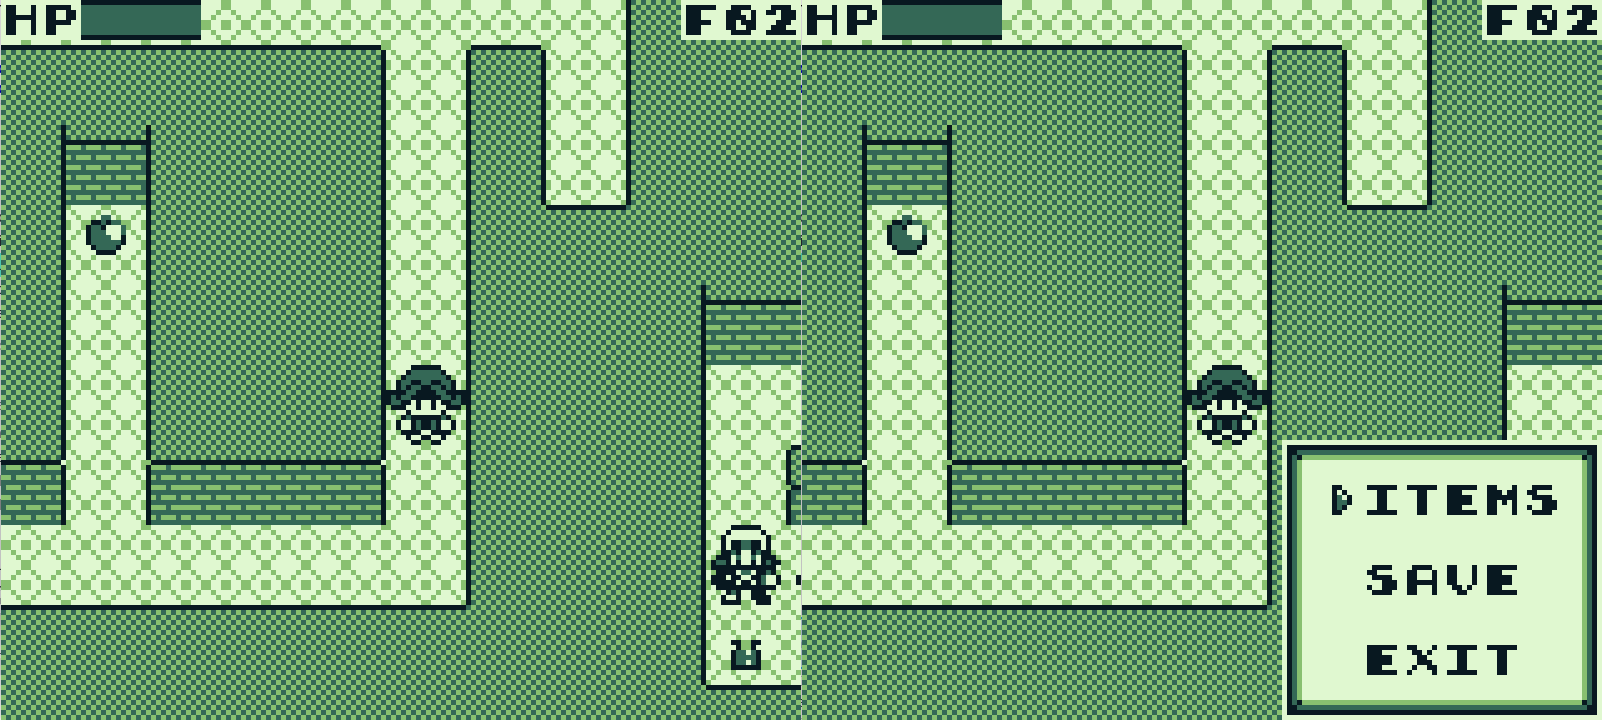
\includegraphics[width=0.8\textwidth]{include/images/desarrollo/fixedhud.png}
\caption{Arreglo Visual Ventanas Emergentes}
\label{figure:hudfix}
\end{figure}

\subsection{Mejoras en el Flujo de Juego}

Las mejoras que se van a implementar son dos: el radio de visión de los enemigos y su velocidad.
\\ \\
Implementar el rango de visión es sencillo: dado un valor máximo, comprobamos si las coordenadas X e Y del jugador se encuentran dentro de ese radio respecto al enemigo. Como las comprobaciones no van solamente en una dirección, tendremos primero que hacer la resta de ambos y ver si da acarreo. En caso contrario le restamos el radio de visión máximo. Si el resultado ha vuelto ha dar acarreo o 0, significa que está dentro del rango de visión en ese eje.

\begin{lstlisting}[caption={Rango de Visión en los Enemigos}, label={code:sightradius}]
	[...]

	ld 	 b, a 															; B = Coordenada X del jugador

	[...]

	ld 	 d, a 															; D = Coordenada X del enemigo
	sub  b
	jr 	 c, ai_see_player_swap_x 	 				; Si hay carry significa que la X del jugador es mayor.

	; Si la coordenada del jugador no es mayor, comprobamos si está dentro del rango.
	sub  SIGHT_RADIUS
	jr 	 c, ai_see_player_y 			; Si está dentro del rango pasamos a comprobar la Y.
	jr 	 z, ai_see_player_y

	jr 	 ai_see_player_unsuccess 	; Si no está dentro del rango devolvemos falso.
	
	[...]
	
ai_see_player_swap_x:
	
	; Si la coordenada X del jugador es mayor, llegamos aquí. Realizamos la operación inversa y le restamos el rango de visión.	
	
	ld 	 a, b
	sub  d
	sub  SIGHT_RADIUS
	jr 	 c, ai_see_player_y
	jr 	 z, ai_see_player_y
	jr 	 ai_see_player_unsuccess	
	
\end{lstlisting}

El método nos devuelve falso si el enemigo no es capaz de ver al jugador, y 1 en caso contrario. De esta manera no vamos a tener enemigos persiguiéndonos de manera constante independientemente de donde nos encontremos.
\\ \\
La segunda mejora da mucho juego, y se trata de la velocidad de cada enemigo. Esta velocidad va a ser distinta para cada uno de ellos, y va a dotar al juego de más posibilidades a la hora que el jugador tome una decisión u otra.
\\ \\
Esto es muy sencillo y lo hemos hecho ya en algún otro momento a lo largo del desarrollo. Lo único que tenemos que hacer es añadir un byte más al tamaño de los enemigos que simbolice esta velocidad. Si queremos que el enemigo se mueva un tercio del jugador, lo que hará será moverse tres casillas y luego dejar pasar un turno. Con esto en mente, por ejemplo, podríamos ponerle a ese enemigo que su velocidad es 3. Por cada turno que pase, esa velocidad se decrementará y al llegar a 0 se reiniciará y es cuando hará el parón. Esto quiere decir que, la velocidad de este enemigo en específico, es de 3/4, ya que se mueve 3 de cada 4 casillas.
\\ \\
Como solamente estamos usando un byte, este mismo va a ser el que nos aporte la información del valor inicial y el valor actual. Si un byte son 8 bits, podemos usar los 4 primeros para uno y los 4 siguientes para otro. Esto nos impide tener velocidades mayores de 15, pero creo que es completamente innecesario.
\\ \\
La comprobación de este valor, finalmente, lo haremos en la toma de decisiones del enemigo. Si no puede atacar al jugador, comprobaremos si se puede mover según su velocidad.

\begin{lstlisting}[caption={Velocidad de los Enemigos}, label={code:velocity}]
	ld 	 e, en_velocity
	call EM_GET_ENEMY_VARIABLE 				; Obtenemos velocidad del enemigo
	ld 	 d, a 														; La guardamos en D y la decrementamos
	dec  a
	jr 	 c, .decide_move_keep 						; Si da acarreo (== 0) podemos movernos

	ld 	 a, d 														; Obtenemos los 4 bits de la velocidad actual
	and  %00001111
	dec  a 														; Decrementamos el valor
	jr 	 nz, .decide_move_update_velocity 	; Si no da 0 significa que podemos movernos

	; En caso contrario tenemos que resetear la velocidad
	
	ld 	 a, d
	and  %11110000 										; Obtenemos los 4 bits que nos da el valor por defecto.
	ld 	 d, a 														; Lo guardamos en D
	swap a 													; Hacemos un swap al registro a (tendremos %00001111)
	or 	 d 														; Aplicamos una operación de tipo OR
	ld 	 [hl], a 													; Guardamos el valor resultante

	jp 	 .decide_not_m 									; Impedimos el movimiento.
\end{lstlisting}

\subsection{Conclusión}

Esta iteración ha servido para dejar algunas de las tareas secundarias terminadas. Pienso que el trabajo en estas dos semanas ha sido bueno y productivo, y que he conseguido dejar un producto cerrado y bien acabado. El trabajo que queda de aquí en adelante (el poco tiempo que me queda de aquí a la entrega) se va a enfocar en meter más niveles y alguna canción más. En cuanto a inteligencia artificial, por ejemplo, no da tiempo a hacer nada demasiado complejo.

\cleardoublepage


